\documentclass[]{elsarticle} %review=doublespace preprint=single 5p=2 column
%DIF LATEXDIFF DIFFERENCE FILE
%DIF DEL article_springer_alt.tex   Tue Mar 10 16:50:05 2020
%DIF ADD article_springer_neu.tex   Sun Mar  1 14:00:12 2020
%%% Begin My package additions %%%%%%%%%%%%%%%%%%%
\usepackage[hyphens]{url}



\usepackage{lineno} % add
\providecommand{\tightlist}{%
  \setlength{\itemsep}{0pt}\setlength{\parskip}{0pt}}

\usepackage{graphicx}
\usepackage{booktabs} % book-quality tables
%%%%%%%%%%%%%%%% end my additions to header

\usepackage[T1]{fontenc}
\usepackage{lmodern}
\usepackage{amssymb,amsmath}
\usepackage{ifxetex,ifluatex}
\usepackage{fixltx2e} % provides \textsubscript
% use upquote if available, for straight quotes in verbatim environments
\IfFileExists{upquote.sty}{\usepackage{upquote}}{}
\ifnum 0\ifxetex 1\fi\ifluatex 1\fi=0 % if pdftex
  \usepackage[utf8]{inputenc}
\else % if luatex or xelatex
  \usepackage{fontspec}
  \ifxetex
    \usepackage{xltxtra,xunicode}
  \fi
  \defaultfontfeatures{Mapping=tex-text,Scale=MatchLowercase}
  \newcommand{\euro}{€}
\fi
% use microtype if available
\IfFileExists{microtype.sty}{\usepackage{microtype}}{}
\bibliographystyle{elsarticle-harv}
\ifxetex
  \usepackage[setpagesize=false, % page size defined by xetex
              unicode=false, % unicode breaks when used with xetex
              xetex]{hyperref}
\else
  \usepackage[unicode=true]{hyperref}
\fi
\hypersetup{breaklinks=true,
            bookmarks=true,
            pdfauthor={},
            pdftitle={Statistical Inference for inter-arrival times of extreme events in bursty time series},
            colorlinks=false,
            urlcolor=blue,
            linkcolor=magenta,
            pdfborder={0 0 0}}
\urlstyle{same}  % don't use monospace font for urls

\setcounter{secnumdepth}{5}
% Pandoc toggle for numbering sections (defaults to be off)
%DIF 54a54-55
 %DIF > 
 %DIF > 
%DIF -------
% Pandoc header
%DIF PREAMBLE EXTENSION ADDED BY LATEXDIFF
%DIF UNDERLINE PREAMBLE %DIF PREAMBLE
\RequirePackage[normalem]{ulem} %DIF PREAMBLE
\RequirePackage{color}\definecolor{RED}{rgb}{1,0,0}\definecolor{BLUE}{rgb}{0,0,1} %DIF PREAMBLE
\providecommand{\DIFaddtex}[1]{{\protect\color{blue}\uwave{#1}}} %DIF PREAMBLE
\providecommand{\DIFdeltex}[1]{{\protect\color{red}\sout{#1}}}                      %DIF PREAMBLE
%DIF SAFE PREAMBLE %DIF PREAMBLE
\providecommand{\DIFaddbegin}{} %DIF PREAMBLE
\providecommand{\DIFaddend}{} %DIF PREAMBLE
\providecommand{\DIFdelbegin}{} %DIF PREAMBLE
\providecommand{\DIFdelend}{} %DIF PREAMBLE
\providecommand{\DIFmodbegin}{} %DIF PREAMBLE
\providecommand{\DIFmodend}{} %DIF PREAMBLE
%DIF FLOATSAFE PREAMBLE %DIF PREAMBLE
\providecommand{\DIFaddFL}[1]{\DIFadd{#1}} %DIF PREAMBLE
\providecommand{\DIFdelFL}[1]{\DIFdel{#1}} %DIF PREAMBLE
\providecommand{\DIFaddbeginFL}{} %DIF PREAMBLE
\providecommand{\DIFaddendFL}{} %DIF PREAMBLE
\providecommand{\DIFdelbeginFL}{} %DIF PREAMBLE
\providecommand{\DIFdelendFL}{} %DIF PREAMBLE
%DIF HYPERREF PREAMBLE %DIF PREAMBLE
\providecommand{\DIFadd}[1]{\texorpdfstring{\DIFaddtex{#1}}{#1}} %DIF PREAMBLE
\providecommand{\DIFdel}[1]{\texorpdfstring{\DIFdeltex{#1}}{}} %DIF PREAMBLE
\newcommand{\DIFscaledelfig}{0.5}
%DIF HIGHLIGHTGRAPHICS PREAMBLE %DIF PREAMBLE
\RequirePackage{settobox} %DIF PREAMBLE
\RequirePackage{letltxmacro} %DIF PREAMBLE
\newsavebox{\DIFdelgraphicsbox} %DIF PREAMBLE
\newlength{\DIFdelgraphicswidth} %DIF PREAMBLE
\newlength{\DIFdelgraphicsheight} %DIF PREAMBLE
% store original definition of \includegraphics %DIF PREAMBLE
\LetLtxMacro{\DIFOincludegraphics}{\includegraphics} %DIF PREAMBLE
\newcommand{\DIFaddincludegraphics}[2][]{{\color{blue}\fbox{\DIFOincludegraphics[#1]{#2}}}} %DIF PREAMBLE
\newcommand{\DIFdelincludegraphics}[2][]{% %DIF PREAMBLE
\sbox{\DIFdelgraphicsbox}{\DIFOincludegraphics[#1]{#2}}% %DIF PREAMBLE
\settoboxwidth{\DIFdelgraphicswidth}{\DIFdelgraphicsbox} %DIF PREAMBLE
\settoboxtotalheight{\DIFdelgraphicsheight}{\DIFdelgraphicsbox} %DIF PREAMBLE
\scalebox{\DIFscaledelfig}{% %DIF PREAMBLE
\parbox[b]{\DIFdelgraphicswidth}{\usebox{\DIFdelgraphicsbox}\\[-\baselineskip] \rule{\DIFdelgraphicswidth}{0em}}\llap{\resizebox{\DIFdelgraphicswidth}{\DIFdelgraphicsheight}{% %DIF PREAMBLE
\setlength{\unitlength}{\DIFdelgraphicswidth}% %DIF PREAMBLE
\begin{picture}(1,1)% %DIF PREAMBLE
\thicklines\linethickness{2pt} %DIF PREAMBLE
{\color[rgb]{1,0,0}\put(0,0){\framebox(1,1){}}}% %DIF PREAMBLE
{\color[rgb]{1,0,0}\put(0,0){\line( 1,1){1}}}% %DIF PREAMBLE
{\color[rgb]{1,0,0}\put(0,1){\line(1,-1){1}}}% %DIF PREAMBLE
\end{picture}% %DIF PREAMBLE
}\hspace*{3pt}}} %DIF PREAMBLE
} %DIF PREAMBLE
\LetLtxMacro{\DIFOaddbegin}{\DIFaddbegin} %DIF PREAMBLE
\LetLtxMacro{\DIFOaddend}{\DIFaddend} %DIF PREAMBLE
\LetLtxMacro{\DIFOdelbegin}{\DIFdelbegin} %DIF PREAMBLE
\LetLtxMacro{\DIFOdelend}{\DIFdelend} %DIF PREAMBLE
\DeclareRobustCommand{\DIFaddbegin}{\DIFOaddbegin \let\includegraphics\DIFaddincludegraphics} %DIF PREAMBLE
\DeclareRobustCommand{\DIFaddend}{\DIFOaddend \let\includegraphics\DIFOincludegraphics} %DIF PREAMBLE
\DeclareRobustCommand{\DIFdelbegin}{\DIFOdelbegin \let\includegraphics\DIFdelincludegraphics} %DIF PREAMBLE
\DeclareRobustCommand{\DIFdelend}{\DIFOaddend \let\includegraphics\DIFOincludegraphics} %DIF PREAMBLE
\LetLtxMacro{\DIFOaddbeginFL}{\DIFaddbeginFL} %DIF PREAMBLE
\LetLtxMacro{\DIFOaddendFL}{\DIFaddendFL} %DIF PREAMBLE
\LetLtxMacro{\DIFOdelbeginFL}{\DIFdelbeginFL} %DIF PREAMBLE
\LetLtxMacro{\DIFOdelendFL}{\DIFdelendFL} %DIF PREAMBLE
\DeclareRobustCommand{\DIFaddbeginFL}{\DIFOaddbeginFL \let\includegraphics\DIFaddincludegraphics} %DIF PREAMBLE
\DeclareRobustCommand{\DIFaddendFL}{\DIFOaddendFL \let\includegraphics\DIFOincludegraphics} %DIF PREAMBLE
\DeclareRobustCommand{\DIFdelbeginFL}{\DIFOdelbeginFL \let\includegraphics\DIFdelincludegraphics} %DIF PREAMBLE
\DeclareRobustCommand{\DIFdelendFL}{\DIFOaddendFL \let\includegraphics\DIFOincludegraphics} %DIF PREAMBLE
%DIF LISTINGS PREAMBLE %DIF PREAMBLE
\RequirePackage{listings} %DIF PREAMBLE
\RequirePackage{color} %DIF PREAMBLE
\lstdefinelanguage{DIFcode}{ %DIF PREAMBLE
%DIF DIFCODE_UNDERLINE %DIF PREAMBLE
  moredelim=[il][\color{red}\sout]{\%DIF\ <\ }, %DIF PREAMBLE
  moredelim=[il][\color{blue}\uwave]{\%DIF\ >\ } %DIF PREAMBLE
} %DIF PREAMBLE
\lstdefinestyle{DIFverbatimstyle}{ %DIF PREAMBLE
	language=DIFcode, %DIF PREAMBLE
	basicstyle=\ttfamily, %DIF PREAMBLE
	columns=fullflexible, %DIF PREAMBLE
	keepspaces=true %DIF PREAMBLE
} %DIF PREAMBLE
\lstnewenvironment{DIFverbatim}{\lstset{style=DIFverbatimstyle}}{} %DIF PREAMBLE
\lstnewenvironment{DIFverbatim*}{\lstset{style=DIFverbatimstyle,showspaces=true}}{} %DIF PREAMBLE
%DIF END PREAMBLE EXTENSION ADDED BY LATEXDIFF

\begin{document}
\begin{frontmatter}

  \title{Statistical Inference for inter-arrival times of extreme events in
bursty time series}
    \author[a]{Katharina Hees}
   \ead{hees@statistik.tu-dortmund.de} 
    \DIFdelbegin %DIFDELCMD < 

%DIFDELCMD <     %%%
\DIFdelend \author[b]{Smarak Nayak}
   \ead{smarak.nayak@nab.com.au} 
    \DIFdelbegin %DIFDELCMD < 

%DIFDELCMD <     %%%
\DIFdelend \author[c]{Peter Straka}
   \DIFdelbegin %DIFDELCMD < \ead{p.straka@unsw.edu.au} 
%DIFDELCMD <   

%DIFDELCMD <       %%%
\DIFdelend \DIFaddbegin \ead{straka.ps@gmail.com} 
      \DIFaddend \address[a]{Department of Statistics, TU Dortmund University, Dortmund, Germany}
    \address[b]{National Australia Bank, Melbourne, Australia}
    \address[c]{School of Mathematics and Statistics, UNSW, Sydney, Australia}

  \begin{abstract}
  In many complex systems studied in statistical physics, inter-arrival
  times between events such as solar flares, trades and neuron voltages
  follow a heavy-tailed distribution. The set of event times is
  fractal-like, being dense in some time windows and empty in others, a
  phenomenon which has been dubbed ``bursty''.

  This article proposes a new model for the \emph{inter-exceedance times}
  of events above high thresholds; the threshold exceedances itself are
  modeled via the standard Peaks-Over-Threshold (POT) method. For high
  thresholds and infinite-mean waiting times, we show that the times
  between threshold crossings are Mittag-Leffler distributed, and thus
  form a ``fractional Poisson Process'' which generalizes the standard
  Poisson Process of threshold exceedances. We provide graphical means of
  estimating model parameters and assessing model fit. Along the way, we
  apply our inference method to a real-world bursty time series, and show
  how the memory of the Mittag-Leffler distribution affects the predictive
  distribution for the time until the next extreme event.
  \end{abstract}
   \begin{keyword} heavy tails renewal process extreme value theory peaks over threshold\end{keyword}
 \end{frontmatter}

\hypertarget{introduction}{%
\section{Introduction}\label{introduction}}

Time series displaying temporally inhomogeneous behaviour in terms of
the occurrence of events have received strong interest in the recent
statistical physics literature (\DIFaddbegin \DIFadd{Bagrow and Brockmann, 2013; }\DIFaddend Barabási\DIFaddbegin \DIFadd{,
}\DIFaddend 2005\DIFdelbegin \DIFdel{; Oliveira and Barabási
2005}\DIFdelend ; \DIFdelbegin \DIFdel{Vasquez }\DIFdelend \DIFaddbegin \DIFadd{Karsai }\DIFaddend et al.\DIFdelbegin \DIFdel{2006; Vazquez }\DIFdelend \DIFaddbegin \DIFadd{, 2011; Min }\DIFaddend et al.\DIFdelbegin \DIFdel{2007; }\DIFdelend \DIFaddbegin \DIFadd{, 2011; Oliveira and Barabási,
2005; }\DIFaddend Omi and Shinomoto\DIFaddbegin \DIFadd{, }\DIFaddend 2011\DIFdelbegin \DIFdel{;
Min, Goh, and Vazquez 2011}\DIFdelend ; \DIFdelbegin \DIFdel{Karsai }\DIFdelend \DIFaddbegin \DIFadd{Vasquez }\DIFaddend et al.\DIFdelbegin \DIFdel{2011; Bagrow and Brockmann
2013}\DIFdelend \DIFaddbegin \DIFadd{, 2006; Vazquez et al.,
2007}\DIFaddend ). They have been observed in the context of earthquakes, sunspots,
neuronal activity and human communication (see Karsai et al.\DIFaddbegin \DIFadd{, }\DIFaddend 2012;
\DIFdelbegin \DIFdel{Vajna, Tóth, and Kertész 2013; }\DIFdelend Meerschaert and Stoev\DIFaddbegin \DIFadd{, }\DIFaddend 2008 for a list of references\DIFaddbegin \DIFadd{; Vajna et al.,
2013}\DIFaddend ). Such time series exhibit high activity in some `bursty'
intervals, which alternate with other, quiet intervals. Although several
mechanisms are plausible explanations for bursty behaviour (most
prominently self-exciting point process by Hawkes (1971)), there seems
to be one salient feature which very typically indicates the departure
from temporal homogeneity: a heavy-tailed distribution of waiting times
(\DIFdelbegin \DIFdel{Vasquez et al. 2006; }\DIFdelend Karsai et al.\DIFaddbegin \DIFadd{, }\DIFaddend 2012; Vajna \DIFdelbegin \DIFdel{, Tóth, and Kertész
}\DIFdelend \DIFaddbegin \DIFadd{et al., }\DIFaddend 2013\DIFaddbegin \DIFadd{; Vasquez et al., 2006}\DIFaddend ). As we
show below in simulations, a simple renewal process with heavy-tailed
waiting times can capture this type of dynamics. For many systems, the
renewal property is appropriate; a simple test of the absence of
correlations in a succession of waiting times can be undertaken by
randomly reshuffling the waiting times (Karsai et al.\DIFaddbegin \DIFadd{, }\DIFaddend 2012).

Often a magnitude, or mark can be assigned to each event in the renewal
process, such as for earthquakes, solar flares or neuron voltages. The
Peaks-Over-Threshold model (POT, see e.g.~Coles\DIFaddbegin \DIFadd{, }\DIFaddend 2001) applies a
threshold to the magnitudes, and fits a Generalized Pareto distribution
to the threshold exceedances. A commonly made assumption in POT models
is that times between events are either fixed or light-tailed, and this
entails that the threshold crossing times form a Poisson process (``On
the Exceedance Point Process for a Stationary Sequence\DIFaddbegin \DIFadd{,}\DIFaddend '' 1988). Then as
one increases the threshold and thus decreases the threshold crossing
probability \DIFdelbegin \DIFdel{\(p\)}\DIFdelend \DIFaddbegin \DIFadd{\(p_{\ell}\)}\DIFaddend , the Poisson process is rarefied, i.e.~its
intensity decreases \emph{linearly} with \DIFdelbegin \DIFdel{\(p\) }\DIFdelend \DIFaddbegin \DIFadd{\(p_{\ell}\) }\DIFaddend (see e.g.~Beirlant
et al.\DIFaddbegin \DIFadd{, }\DIFaddend 2006).

As will be shown below, in the heavy-tailed waiting time scenario
threshold crossing times form a \emph{fractional Poisson process}
(Laskin\DIFaddbegin \DIFadd{, }\DIFaddend 2003; Meerschaert \DIFdelbegin \DIFdel{, Nane, and Vellaisamy }\DIFdelend \DIFaddbegin \DIFadd{et al., }\DIFaddend 2011), which is a renewal process
with Mittag-Leffler distributed waiting times. The family of
Mittag-Leffler distributions nests the exponential distribution (Haubold
\DIFdelbegin \DIFdel{, Mathai, and Saxena }\DIFdelend \DIFaddbegin \DIFadd{et al., }\DIFaddend 2011), and hence the fractional Poisson process generalizes the
standard Poisson process. Again as the threshold size increases and the
threshold crossing probability \DIFdelbegin \DIFdel{\(p\) }\DIFdelend \DIFaddbegin \DIFadd{\(p_{\ell}\) }\DIFaddend decreases, the fractional
Poisson process is rarefied: The scale parameter of the Mittag-Leffler
inter-arrival times of threshold crossing times increases, but
\emph{superlinearly}; see the Theorem below.

Maxima of events which occur according to a renewal process with
heavy-tailed waiting times have been studied under the names
``Continuous Time Random Maxima process'' (CTRM) (Benson \DIFdelbegin \DIFdel{, Schumer, and
Meerschaert }\DIFdelend \DIFaddbegin \DIFadd{et al., }\DIFaddend 2007;
\DIFdelbegin \DIFdel{Meerschaert and Stoev 2008; }\DIFdelend Hees and Scheffler\DIFdelbegin \DIFdel{2018b}\DIFdelend , 2018a\DIFaddbegin \DIFadd{, 2018b; Meerschaert and Stoev, 2008}\DIFaddend ),
``Max-Renewal process'' (\DIFdelbegin \DIFdel{Silvestrov }\DIFdelend \DIFaddbegin \DIFadd{Basrak and Špoljarić, 2015; Silvestrov, }\DIFaddend 2002;
Silvestrov and Teugels\DIFaddbegin \DIFadd{, }\DIFaddend 2004\DIFdelbegin \DIFdel{; Basrak and Špoljarić 2015}\DIFdelend ), and ``Shock process'' (\DIFaddbegin \DIFadd{Anderson, 1987;
}\DIFaddend Esary and Marshall\DIFaddbegin \DIFadd{, }\DIFaddend 1973; \DIFaddbegin \DIFadd{Gut and Hüsler, 1999; }\DIFaddend Shanthikumar and Sumita\DIFdelbegin \DIFdel{1983,
1984}\DIFdelend ,
1985\DIFdelbegin \DIFdel{; Anderson 1987;
Gut and Hüsler 1999}\DIFdelend \DIFaddbegin \DIFadd{, 1984, 1983}\DIFaddend ). The existing literature focuses on probabilistic
results surrounding these models. In this work, however, we introduce a
method of inference for this type of model, which is seemingly not
available in the literature.

We review the marked renewal process in Section 2, and derive a scaling
limit theorem for inter-exceedance times in Section 3. We give a
statistical procedure to estimate model parameters via stability plots
in Section 5, but to set the stage we first discuss inference for the
Mittag-Leffler distribution in Section 4. A simulation study of the
effectiveness of our statistical procedure is given in Section 6. In
Section 7 we apply our method to a real data set. In Section 8, we
discuss the memory property of the Mittag-Leffler distribution, and how
it affects the predictive distribution for the time until the next
threshold crossing event. Finally we close with a discussion and
conclusion in Section 9. For all statistical computations we have used R
(R Core Team\DIFaddbegin \DIFadd{, }\DIFaddend 2018). All code and data used for the analysis in this
article has been organized into an R package \texttt{CTRE}
(\url{https://github.com/strakaps/CTRE}). The source code for the
figures generated in this manuscript is available online at
\url{https://github.com/strakaps/bursty-POT}.

\hypertarget{continuous-time-random-exceedances-ctre}{%
\section{Continuous Time Random Exceedances
(CTRE)}\label{continuous-time-random-exceedances-ctre}}

As a model for extreme observations, we use a Marked Renewal Process
(MRP):

\begin{description}
\item[\textbf{Definition (MRP):}]
Let \((W,J), (W_1, J_1), (W_2, J_2), \ldots\) be i.i.d. pairs of random
variables, where the \(W_k > 0\) are interpreted as the \emph{waiting
times} and \DIFdelbegin \DIFdel{\(J_k \in [x_L, x_R]\) }\DIFdelend \DIFaddbegin \DIFadd{\(J_k \in \mathbb{R}\) }\DIFaddend as the \emph{event magnitudes}\DIFdelbegin \DIFdel{(\(x_L \in [-\infty, +\infty), x_R \in (-\infty, +\infty]\))}\DIFdelend . If
\(W\) and \(J\) are independent, the Marked Renewal Process is said to
be \emph{uncoupled}.
\end{description}

\DIFaddbegin \DIFadd{In the following we denote with \(x_L \in [-\infty, +\infty)\) and
\(x_R \in (-\infty, +\infty]\)) the left and right endpoint of the
distribution of \(J\). }\DIFaddend We assume that the \(k\)-th magnitude \(J_k\)
occurs at time \(T_k = W_1 + \ldots + W_k\). Based on an MRP, we define
the Continuous Time Random Exceedance model (CTRE) as follows:

\begin{description}
\item[\textbf{Definition (CTRE):}]
Given a threshold \(\ell \in (x_L, x_R)\), consider the stopping time
\[\tau(\ell) := \min\{k: J_k > \ell\},\quad \ell \in (x_L, x_R).\]
Define the pair of random variables \((X(\ell), T(\ell))\) via
\[X(\ell) = J_{\tau(\ell)} - \ell, \quad 
T(\ell) = \sum_{k=1}^{\tau(\ell)} W_k.\] By restarting the MRP at
\(\tau(\ell)\), inductively define the two i.i.d. sequences
\(T(\ell,n)\) and \(X(\ell, n)\), \(n \in \mathbb N\), called the
``inter-arrival times'' and the ``exceedances'', respectively. The pair
sequence \DIFdelbegin \DIFdel{\((T(\ell, n), W(\ell, n))_{n \in \mathbb N}\) }\DIFdelend \DIFaddbegin \DIFadd{\((X(\ell, n), T(\ell, n))_{n \in \mathbb N}\) }\DIFaddend is called a
Continuous Time Random Exceedance model (CTRE). If the underlying MRP is
uncoupled, then the CTRE is also called uncoupled.
\end{description}

\begin{figure}

{\centering 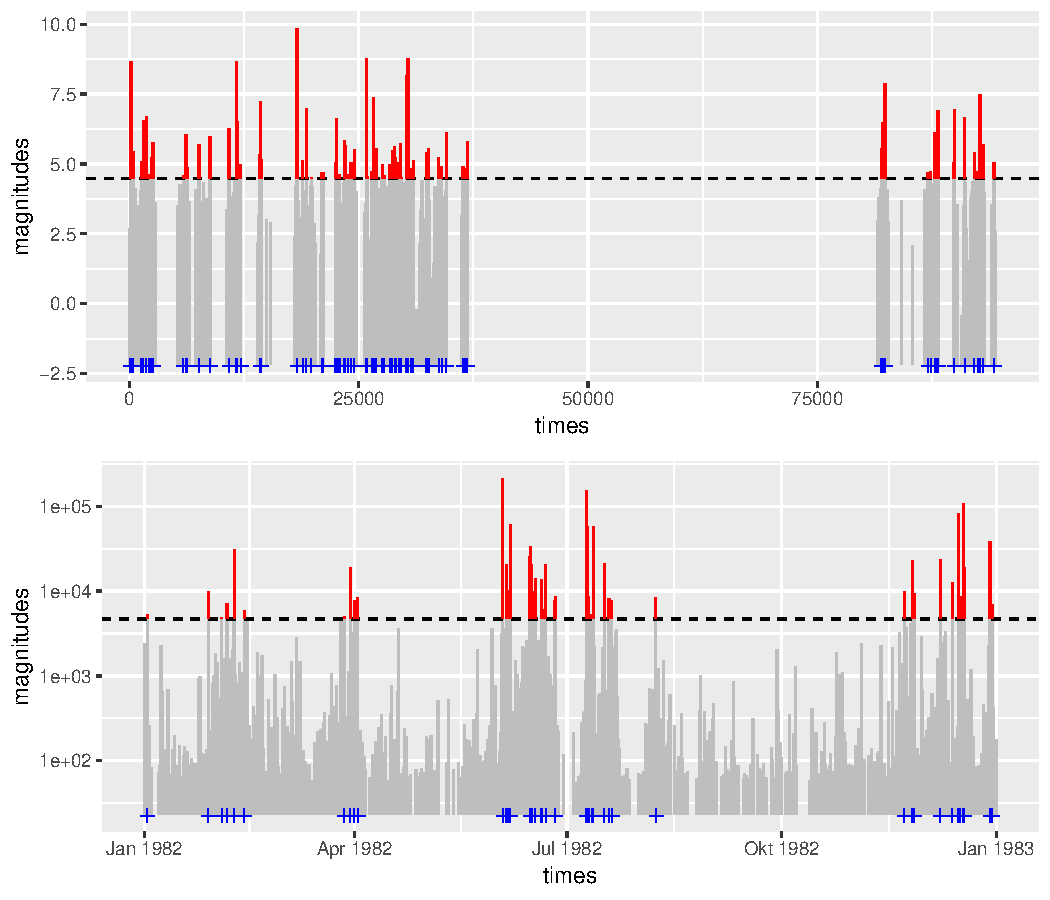
\includegraphics[width=0.7\linewidth]{article_springer_files/figure-latex/thresholdedBursty-1} 

}

\caption{\label{fig:thresholdedBursty} Exceedances (red) and times until Exceedance (durations between blue crosses) for a given threshold $\ell$ (dashed line). Upper picture: Simulated data with stable distributed waiting times. Lower picture: Solar flares during 1982.}\label{fig:thresholdedBursty}
\end{figure}

In this article, we restrict ourselves to the uncoupled case, where
\(W\) and \(J\) are independent. Then the two sequences
\(X(\ell, n)_{n \in \mathbb N}\) and \(T(\ell, n)_{n \in \mathbb N}\)
are independent as well. To see why, note that \(X(\ell)\) is, in
distribution, simply equal to \DIFdelbegin \DIFdel{\(J | J > \ell\)}\DIFdelend \DIFaddbegin \DIFadd{\(J - \ell | J > \ell\)}\DIFaddend , independent of
any waiting time \(W_k\).\\
\DIFaddbegin \DIFadd{We assume for the rest of the article, that the magnitudes
\((J_i)_{i \in \mathbb{N}}\) belong to the the max-domain of attraction
of some non-degenerate distribution. This means there exist \(a_n>0\)
and \(d_n \in \mathbb{R}\) such that
}\[ \DIFadd{a_n^{-1}(J_1 \vee \ldots \vee J_n -d_n) \Rightarrow A \text{ as } n \rightarrow \infty.}\]
\DIFadd{Hence, the distribution of \(A\) is a generalized extreme value
distribution (GEV) which distribution function is given by
}\[ \DIFadd{F(x;\xi) = \begin{cases}\exp(-(1+\xi x)^{-1/\xi}) & \xi\neq0 \\ \exp(-\exp(-x)) & \xi = 0\end{cases}.}\]
\DIFadd{The GEV is subdivided into the Gumbel (\(\xi=0\)), the Weibull
(\(\xi<0\)) and the Fr'echet (\(\xi>0\)) family of distributions.
}

\DIFaddend Figure \ref{fig:thresholdedBursty} shows a simulated dataset in the top
panel, where \(W\) has a stable distribution with tail parameter
\(\beta =\) 0.8 (and skewness \(1\) and location \(0\)), and where \(J\)
is from a standard Gumbel distribution. In the bottom panel, we plot a
time series of solar flare intensities derived from a NASA dataset
(Dennis et al.\DIFaddbegin \DIFadd{, }\DIFaddend 1991) which we will later examine more closely (see
Section 7). Clearly, the simulated data exhibit long intervals
\emph{without any} events, whereas in the real-world dataset events
appear continuously. The threshold exceedances, however, appear to have
visually similar statistical behaviour in both models. Observations
below a threshold are commonly discarded in Extreme Value Theory (POT
approach); likewise, the CTRE model interprets these observations as
noise and discards them.

\hypertarget{sec:scaling}{%
\section{Scaling limit of Exceedance Times}\label{sec:scaling}}

In this section we state and prove the key theorem\DIFdelbegin \DIFdel{, see below}\DIFdelend . For an accessible
introduction to regular variation and stable limit theorems, we
recommend the book by \DIFdelbegin \DIFdel{Mark M }\DIFdelend Meerschaert and Sikorskii (2012).

\begin{description}
\item[\textbf{Theorem:}]
Let the waiting times \DIFdelbegin \DIFdel{\(J_k\) }\DIFdelend \DIFaddbegin \DIFadd{\(W_k\) }\DIFaddend be in the domain of attraction of a
positively skewed sum-stable law with stability parameter
\(0 < \beta < 1\); more precisely, \begin{align} \label{eq:stability}
\frac{W_1 + \ldots + W_n}{b(n)} \overset{d}{\longrightarrow} D, 
\quad n \to \infty
\end{align} for a function \(b(n)\) which is regularly varying at
\(\infty\) with parameter \(1/\beta\), and where
\(\mathbf E[\exp(-sD)] = \exp(-s^\beta)\). Write
\DIFdelbegin \DIFdel{\(p := \mathbf P(J > \ell)\)}\DIFdelend \DIFaddbegin \DIFadd{\(p_{\ell} := \mathbf P(J > \ell)\)}\DIFaddend . Then the weak convergence \[
\frac{T(\ell)} {b(1/p\DIFaddbegin \DIFadd{_{\ell}}\DIFaddend )} \to \DIFdelbegin \DIFdel{W}\DIFdelend \DIFaddbegin \DIFadd{Z}\DIFaddend _\beta \quad \text{ as } \quad \ell \uparrow x_R
\] holds, where the Mittag-Leffler random variable \DIFdelbegin \DIFdel{\(W_\beta\) }\DIFdelend \DIFaddbegin \DIFadd{\(Z_\beta\) }\DIFaddend is
defined on the positive real numbers via \[
\mathbf E[\exp(\DIFdelbegin \DIFdel{-sW}\DIFdelend \DIFaddbegin \DIFadd{-sZ}\DIFaddend _\beta)] = \frac{1}{1+s^\beta}.
\]
\end{description}

\emph{Proof of Theorem:} We interpret the threshold crossing time
\(T(\ell)\) as the hitting time of the underlying CTRM (Continuous Time
Random Maxima) or ``max-renewal process'', and then utilize a result by
Meerschaert and Stoev (2008). The running maximum process is defined as
\[
M(c) := J_1 \vee \ldots \vee J_{\lfloor c \rfloor},
\] and since we assume that the \(J_k\) have a continuous distribution,
there exist norming functions \(a(c)\) and \(d(c)\) such that \[
\mathbf P\left[ \frac{M(c) - d(c)}{a(c)} \le \ell^* \right] 
\longrightarrow F(\ell^*), \quad \DIFdelbegin \DIFdel{t }\DIFdelend \DIFaddbegin \DIFadd{c }\DIFaddend \to \infty
\] where \(F\) is a generalized extreme value distribution, and
\(\ell^*\) is any value from the support of \(F\). The CTRM process is
then defined via \[
V(t) = M(N(t)), \quad t \ge 0
\] where \(N(t)\) is the renewal process associated with the waiting
times \(W_k\): \[
N(t) = \max\{n: W_1 + \ldots + W_n \le t\}.
\] Now a key observation is that \[
T(\ell) = \inf\{t: V(t) > \ell\}, 
\] and that
\DIFdelbegin \[
\DIFdel{T(\ell) > t \quad \text{ if and only if } \quad V(t) \le \ell.
}\]%DIFAUXCMD
\DIFdelend \DIFaddbegin 

\begin{align}
\DIFadd{T(\ell) > t \quad \text{ if and only if } \quad V(t) \le \ell. \label{inverserelat}
}\end{align}\DIFaddend 
\DIFaddbegin 

\DIFaddend By (Theorem 3.1, Meerschaert and Stoev\DIFaddbegin \DIFadd{, }\DIFaddend 2008), we have the stochastic
process convergence
\DIFdelbegin \[
\DIFdel{\frac{V(ct) - d(\tilde b(c))}{a(\tilde b(c))} 
\stackrel{d}{\longrightarrow} Y(t), \quad t > 0.
}\]%DIFAUXCMD
\DIFdelend \DIFaddbegin 

\begin{align}
\DIFadd{\frac{V(ct) - d(\tilde b(c))}{a(\tilde b(c))} 
\stackrel{d}{\longrightarrow} Y(t),  \quad c \to \infty, \label{TheoMS}
}\end{align}\DIFaddend 
\DIFaddbegin 

\DIFadd{for \(t > 0\), }\DIFaddend where \(Y(t)\) is a time-changed (``subordinated'')
extremal process, and where \(\tilde b(c)\) is a regularly varying
norming function which is \emph{inverse} to \(b(c)\), in the sense that
\(b(\tilde b(c)) \sim c \sim \tilde b(b(c))\) \DIFdelbegin \DIFdel{.
}\DIFdelend \DIFaddbegin \DIFadd{(Bingham et al., 1989).
}\DIFaddend 

Without loss of generality, we choose \(\ell^*\) such that
\(F(\ell^*) = 1/e\), and let
\(\ell = a(\tilde b(c)) \ell^* + d(\tilde b(c))\). We may then calculate
\[
\mathbf P\left[ \DIFdelbegin \DIFdel{\frac{T(\ell)}{b(1/p)} }\DIFdelend \DIFaddbegin \DIFadd{\frac{T(\ell)}{b(1/p_{\ell})} }\DIFaddend > t \right]
= \mathbf P[T(\ell) > b(1/p\DIFaddbegin \DIFadd{_{\ell}}\DIFaddend ) t]
= \mathbf P[V(ct) \le \ell]
\] where we have substituted \DIFdelbegin \DIFdel{\(c = b(1/p)\). Moreover}\DIFdelend \DIFaddbegin \DIFadd{\(c = b(1/p_{\ell})\) and used
}\eqref{inverserelat}\DIFadd{. Moreover, we receive due to the convergence in
}\eqref{TheoMS} \DIFaddend \[
\mathbf P[V(ct) \le \ell]
= \mathbf P\left[ \frac{V(ct) - d(\tilde b(c))}{a(\tilde b(c))} 
\le \frac{\ell - d(\tilde b(c))}{a(\tilde b(c))} \right]
\longrightarrow \mathbf P\left[ Y(t) \le \ell^* \right] \DIFaddbegin \DIFadd{,  }\quad \DIFadd{c }\to \DIFadd{\infty,
}\DIFaddend \] \DIFaddbegin \DIFadd{for \(t>0\). }\DIFaddend Defining the hitting time of level \(\ell^*\) by
\(Y(t)\) as \(\xi_{\ell^*} := \inf\{t: Y(t) > \ell^*\}\), we then have
\[
P\left[ Y(t) \le \ell^* \right] = \mathbf P[\xi_{\ell^*} > t] 
= \mathbf P[(-\log F(\ell^*))^{-1/\beta} X^{1/\beta} D > t]
\] by (Proposition 4.2, Meerschaert and Stoev\DIFaddbegin \DIFadd{, }\DIFaddend 2008), where \(X\) is an
exponential random variable with mean \(1\). Using (Theorem 19.1,
Haubold \DIFdelbegin \DIFdel{, Mathai, and Saxena }\DIFdelend \DIFaddbegin \DIFadd{et al., }\DIFaddend 2011), we see that
\(X^{1/\beta} D \sim {\rm ML}(\beta, 1)\), concluding the proof. \qed  

For a scale parameter \(\sigma > 0\), we write
\({\rm ML}(\beta, \sigma)\) for the distribution of \DIFdelbegin \DIFdel{\(\sigma W_\beta\)}\DIFdelend \DIFaddbegin \DIFadd{\(\sigma Z_\beta\)}\DIFaddend .
The Mittag-Leffler distribution with parameter \(\beta \in (0,1]\) is a
heavy-tailed positive distribution for \(\beta < 1\), with infinite
mean. However, as \(\beta \uparrow 1\), \({\rm ML}(\beta, \sigma)\)
converges weakly to the exponential distribution \({\rm Exp}(\sigma)\)
with mean \(\sigma\). This means that although its moments are all
infinite, the Mittag-Leffler distribution may (if \(\beta\) is close to
1) be indistinguishable from the exponential distribution, for the
purposes of applied statistics.
\DIFaddbegin 

\DIFadd{We caution the reader that, somewhat confusingly, there is another
distribution called the ``light-tailed'' Mittag-Leffler distribution.
This is in fact the limiting distribution of the renewal process
\(N(t)\) above (see Meerschaert and Scheffler (2004)). }\DIFaddend For a detailed
reference on the Mittag-Leffler distribution, see e.g.~ Haubold \DIFdelbegin \DIFdel{, Mathai, and Saxena
}\DIFdelend \DIFaddbegin \DIFadd{et al.
}\DIFaddend (2011), and for algorithms, see e.g.~the R package
\texttt{MittagLeffleR} (Gill and Straka\DIFaddbegin \DIFadd{, }\DIFaddend 2017).

\begin{description}
\item[\textbf{Remark:}]
If \(\beta = 1\), the result of the Theorem above is standard, see e.g.~
Equation (2.2) in Gut and Hüsler (1999). In Anderson (1987) a similar
result is shown with a different choice of scaling constant.
\DIFaddbegin \item[\textbf{\DIFadd{Remark:}}]
\DIFadd{When \(0 < \beta < 1\), the renewal process \(N(t)\) is }\emph{\DIFadd{not
stationary}}\DIFadd{, and hence the results by (``On the Exceedance Point Process
for a Stationary Sequence,'' 1988) on the exceedances of stationary
sequences do not apply.
}\DIFaddend \end{description}

\hypertarget{sec:ML}{%
\section{Model Choice and inference for the Mittag-Leffler
distribution}\label{sec:ML}}

The classical POT approach is based on the fact that exceedances above a
high \DIFdelbegin \DIFdel{threshhold }\DIFdelend \DIFaddbegin \DIFadd{threshold }\DIFaddend are asymptotically GPD distributed, hence a GPD
distribution is fitted to the exceedances above a high enough \DIFdelbegin \DIFdel{threshhold}\DIFdelend \DIFaddbegin \DIFadd{threshold}\DIFaddend .
Due to the Theorem in the last Section we know that for high thresholds
the times between exceedances are asymptotically Mittag-Leffler
distributed in case of heavy-tailed waiting times between the
observations. Hence, before we talk about inference for the exceedances
in the next section, we discuss inference for Mittag-Leffler
distributions.

Historically, the first method proposed for the estimation of the
Mittag-Leffler distribution parameters was the fractional moment
estimator by Kozubowski (2001). Unlike the first moments, the fractional
moments of order \(p\) for \(p<\beta\) exist and are tractable. One
drawback of this method is that constant priors for the tail parameter
are needed for the calculation of the estimates. Cahoy \DIFdelbegin \DIFdel{, Uchaikin, and
Woyczynski }\DIFdelend \DIFaddbegin \DIFadd{et al. }\DIFaddend (2010)
proposed a moment estimator of the log-transformed data, which does not
require any prior. Furthermore, they performed simulation studies
illustrating that the log-moment outperforms the fractional moment
estimator with respect to bias and root mean squared error (RMSE).

Due to the form of the density function of a Mittag-Leffler distribution
there exists no closed form for the Maximum Likelihood estimator (MLE).
In the R Package \texttt{MittagLeffleR} (Gill and Straka\DIFaddbegin \DIFadd{, }\DIFaddend 2017), Maximum
Likelihood estimation is implemented via numerical optimization. The MLE
slightly outperforms the log-moment estimator regarding bias and RMSE
for big enough sample sizes, but is extremely \DIFdelbegin \DIFdel{computational }\DIFdelend \DIFaddbegin \DIFadd{computationally }\DIFaddend intensive.
Figure \ref{fig:MSE} shows that both estimators perform well, even for
small sample sizes.

\begin{figure}

{\centering 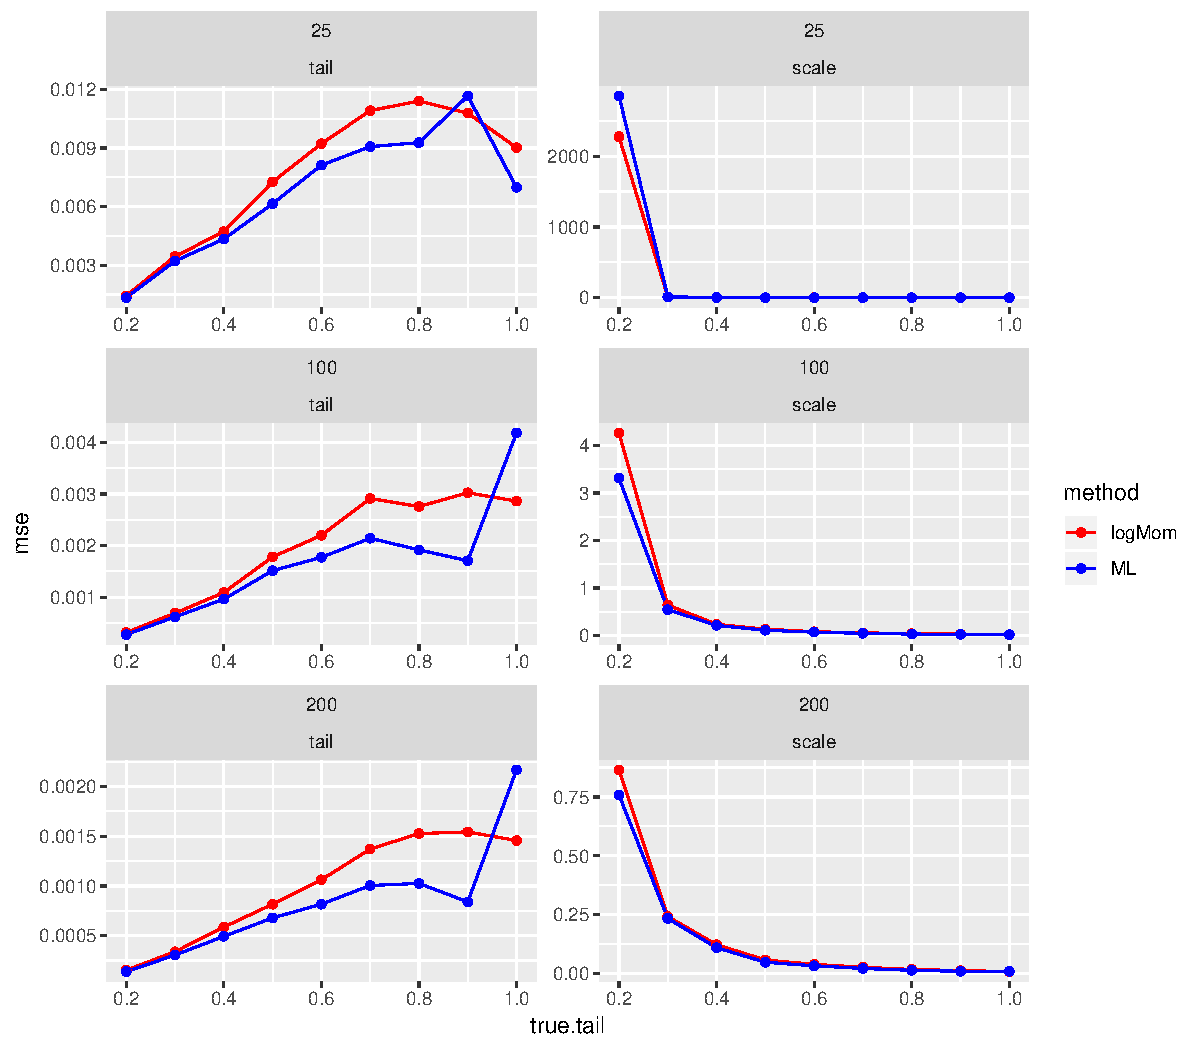
\includegraphics[width=0.9\linewidth]{article_springer_files/figure-latex/MSE-1} 

}

\caption{\label{fig:MSE} MSE for the estimation of tail (left column) and scale (right column) parameters via log-moment estimator and \DIFdelbeginFL \DIFdelFL{mle }\DIFdelendFL \DIFaddbeginFL \DIFaddFL{MLE }\DIFaddendFL of a Mittag-Leffler sample with varying sample size n=25, 100, 200, varying tails on the x-axis and fixed scale equal to one.}\label{fig:MSE}
\end{figure}

Since the Mittag-Leffler distribution is heavy-tailed, many researchers
would intuitively give the highest importance to the tail behaviour of
the distribution. Of course, one can also use established tail exponent
estimators for the estimation of the parameter \(\beta\) such as the
Hill estimator (Hill\DIFaddbegin \DIFadd{, }\DIFaddend 1975) based on the \(r+1\) upper order statistics
\begin{align}\DIFdelbegin %DIFDELCMD < \label{eq:hill}
%DIFDELCMD < %%%
\DIFdelend \DIFaddbegin \label{eq:Hill}
\DIFaddend H_{r,n}=\left[ \frac{1}{r} \sum_{i=0}^{r} \log \frac{X_{(i)}}{X_{(r+1)}}\right]^{-1}, 
\end{align} where \(X_{(1)} \geq X_{(2)} \geq \ldots \geq X_{(n)}\)
denote the order statistics in decreasing order of a sequence
\(X_1,\ldots,X_n\). However, these methods are statistically less
efficient since they only use a portion of the information contained in
the data, as mentioned by Kozubowski (2001). Moreover, the \DIFdelbegin \DIFdel{hill
}\DIFdelend \DIFaddbegin \DIFadd{Hill
}\DIFaddend estimator requires a tuning parameter, denoted with \(r\) in
\DIFdelbegin %DIFDELCMD < \eqref{eq:hill}%%%
\DIFdelend \DIFaddbegin \eqref{eq:Hill}\DIFaddend . Additionaly, the estimator only performs reliably well
for distributions close to Pareto (see Resnick\DIFaddbegin \DIFadd{, }\DIFaddend 1997). Figure
\ref{fig:Hillplots} shows Hill plots for Mittag-Leffler simulated data,
with varying sample sizes and tails. To deduce the correct tail
parameter estimates from these plots is virtually impossible. To
estimate the tail parameter of a Mittag-Leffler distribution with the
\DIFdelbegin \DIFdel{hill }\DIFdelend \DIFaddbegin \DIFadd{Hill }\DIFaddend estimator, the sample size has to be much larger and one has to
choose a large tuning parameter \(r\). In case that only events above a
high threshold are recorded, even \(n=1000\) events are unrealistic.
Furthermore the Hill estimator of course completely fails if the
inter-arrival times are \DIFdelbegin \DIFdel{exponential }\DIFdelend \DIFaddbegin \DIFadd{exponentially }\DIFaddend distributed and not heavy-tailed.
We will \DIFdelbegin \DIFdel{comeback }\DIFdelend \DIFaddbegin \DIFadd{come back }\DIFaddend to the problems with the \DIFdelbegin \DIFdel{hill }\DIFdelend \DIFaddbegin \DIFadd{Hill }\DIFaddend estimtator in Section
\ref{Simulationstudy}.

\begin{figure}

{\centering 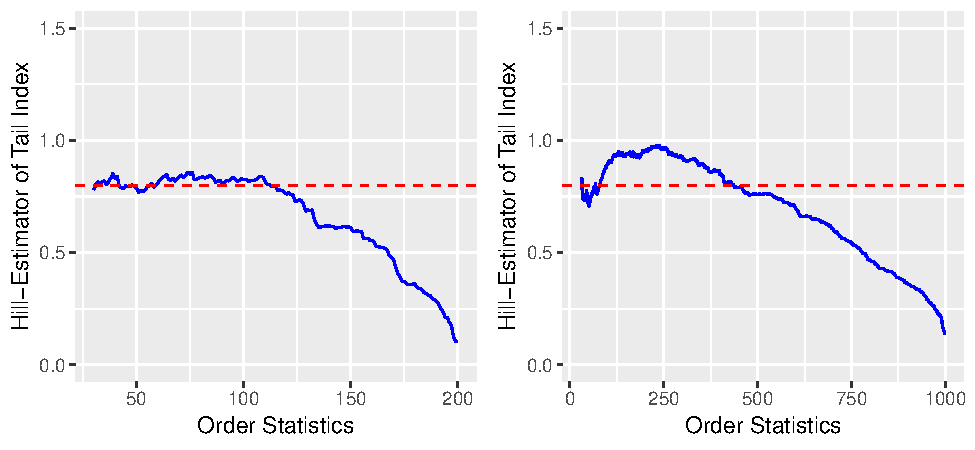
\includegraphics[width=0.9\linewidth]{article_springer_files/figure-latex/Hillplots-1} 

}

\caption{\label{fig:Hillplots} Hillplots for simulated Mittag-Leffler data with true tail 0.8 and sample size 200 (left) and 1000 (right), with number of upper order statics r on which the \DIFdelbeginFL \DIFdelFL{hill }\DIFdelendFL \DIFaddbeginFL \DIFaddFL{Hill }\DIFaddendFL estimator is based on the x-axis. }\label{fig:Hillplots}
\end{figure}

Since the exponential distribution is nested in the Mittag-Leffler
family of distributions, a Likelihood-ratio Test (LRT) seems to be an
appropriate way to choose between a model with exponential and
Mittag-Leffler inter-exceedance times. Although the two models are
nested, the asymptotic distribution is not \(\chi^2_1\)-distributed, and
Wilk's Theorem does not hold: under \(H_0\), the parameter \(\beta\) of
Mittag-Leffler distribution is equal to \(1\), and hence lies on the
boundary of the parameter space \((0,1]\). Instead, a valid approach is
a bootstrapped Likelihood-ratio test (see e.g.~Davison \DIFdelbegin \DIFdel{, Hinkley, and
others }\DIFdelend \DIFaddbegin \DIFadd{et al., }\DIFaddend 1997).
Figure \ref{Fig:LRT} displays the (simulated) power for the bootstrapped
LRT for Mittag-Leffler distributions with varying tail parameters based
on 1000 simulation runs. As expected, the power decreases for tail
parameters close to one, since the Mittag-Leffler distribution converges
as \(\beta \uparrow 1\) to an exponential distribution; it becomes hard
to differentiate a Mittag-Lefller distribution from an exponential.

\begin{figure}

{\centering 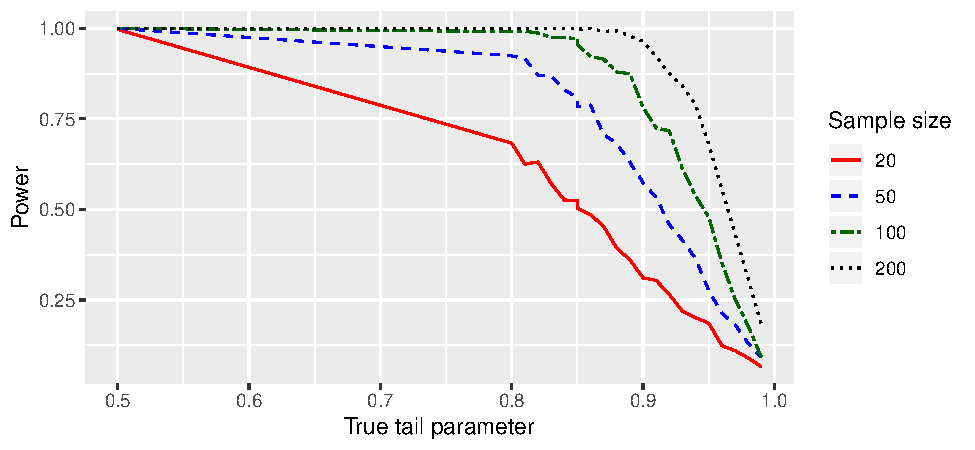
\includegraphics[width=0.9\linewidth]{article_springer_files/figure-latex/LRT_power-1} 

}

\caption{\label{Fig:LRT} Power for bootstrapped LRT for different sample sizes, varying tails and scale parameter equal to 1.}\label{fig:LRT_power}
\end{figure}

\hypertarget{inference-on-exceedance-times}{%
\section{Inference on Exceedance
times}\label{inference-on-exceedance-times}}

The Theorem in Section \ref{sec:scaling} implies that for a high
threshold \(\ell\) we may approximate the distribution of \(T(\ell)\)
with an \DIFdelbegin \DIFdel{\({\rm ML}(\beta, b(1/p))\) }\DIFdelend \DIFaddbegin \DIFadd{\({\rm ML}(\beta, b(1/p_{\ell}))\) }\DIFaddend distribution, where the
function \(b(c)\) varies regularly at \(\infty\) with parameter
\(1/\beta\). Building on the POT (Peaks-Over-Threshold) method, we
propose the following estimation procedure for the distribution of
inter-exceedance time \(T(\ell)\):

\begin{enumerate}
\def\labelenumi{\arabic{enumi}.}
\item
  \DIFdelbegin \DIFdel{For a range of thresholds \(\ell\) near the }\DIFdelend \DIFaddbegin \DIFadd{Extract the \(K\) }\DIFaddend largest order statistics \DIFdelbegin \DIFdel{,
  extract datasets }\DIFdelend \DIFaddbegin \DIFadd{(i.e.~the \(K\) largest
  values, where e.g.~\(K = 300\)) \(X_{(1)}, \ldots, X_{(K)}\) together
  with their timestamps \(T_{(1)}, \ldots, T_{(K)}\).
}\item
  \DIFadd{Choose e.g.~\(K_0 = 5\), and for each \(k\) ranging from \(K_0 +1\) to
  \(K + 1\):
}

  \begin{enumerate}
  \def\labelenumii{\alph{enumii})}
  \tightlist
  \item
    \DIFadd{extract the set \(\mathcal T_k\) }\DIFaddend of exceedance times \DIFdelbegin \DIFdel{\(\{T(\ell, i)\}_i\).
}\DIFdelend \DIFaddbegin \DIFadd{of the
    threshold \(X_{(k)}\)
  }\DIFaddend \item
    \DIFdelbegin \DIFdel{For each choice of threshold \(\ell\), }\DIFdelend fit a Mittag-Leffler distribution to \DIFdelbegin \DIFdel{the resulting dataset \(\{T(\ell, i)\}_i\). This
  results in
    the estimates \(\{\hat\beta(\ell)\}_\ell\) and \(\{\hat \sigma(\ell)\}_\ell\).
  }\DIFdelend \DIFaddbegin \DIFadd{\(\mathcal T_k\), resulting in
    the parameter estimates \(\hat\beta_k\) and \(\hat \sigma_k\).
  }\end{enumerate}
\DIFaddend \item
  Plot \DIFdelbegin \DIFdel{\(\ell\) }\DIFdelend \DIFaddbegin \DIFadd{\(k\) }\DIFaddend vs.~\DIFdelbegin \DIFdel{\(\hat \beta(\ell)\). As \(\ell\) increases towards
  \(x_R\), \(\hat \beta(\ell)\) }\emph{\DIFdel{stabilizes}} %DIFAUXCMD
\DIFdel{around a constant
  \(\hat \beta\). Use \(\hat \beta\) as
  an estimate for the tail
  parameter \(\beta\) of the Mittag-Leffler distribution of exceedance
  times.
}\DIFdelend \DIFaddbegin \DIFadd{\(\hat \beta_k\). To the right, as
  \(k \downarrow K_0\), the asymptotics are off and bias is high. To the
  left (high threshold), data are scarce and variance is high. Choose a
  region of }\emph{\DIFadd{stability}} \DIFadd{in the middle for a parameter estimate
  \(\hat \beta\).
}\DIFaddend \item
  \DIFdelbegin \DIFdel{Approximate \(p \approx |\{k: J_k > \ell\}| / n\). Recall that
  \(b(c)\) is regularly varying with parameter \(1/\beta\), and hence
  has the representation \(b(c) = L(c) c^{1/\beta}\) for some slowly
  varying function \(L(c)\).
Assuming that the variation of \(L(c)\) is
  negligible, we hence plot \(\ell\)
  }\DIFdelend \DIFaddbegin \DIFadd{Plot \(k\) }\DIFaddend vs.~\DIFdelbegin \DIFdel{\(p^{1/\hat \beta} \hat \sigma(\ell)\). Again as \(\ell\)
  increases towards \(x_R\), \(p^{1/\hat \beta} \hat \sigma(\ell)\) is
  expected to stabilize around a constant }\DIFdelend \DIFaddbegin \DIFadd{\(k^{1/\hat \beta} \hat \sigma_k\). Where the plot
  stabilizes as \(k \downarrow K_0\), define the value
  }\DIFaddend \(\hat \sigma_0\).
\DIFdelbegin \DIFdel{We then use
  \(p^{-1/\hat \beta} \hat \sigma_0\) as an estimate of the scale
  parameter of the
Mittag-Leffler distribution of exceedance times for
  the level \(\ell\).
}\DIFdelend \end{enumerate}

\DIFdelbegin \DIFdel{The above approach benefits from the following practical adjustments
(compare with Figure \ref{fig:flares}): }%DIFDELCMD < 

%DIFDELCMD < \begin{itemize}
\begin{itemize}%DIFAUXCMD
%DIFDELCMD < \item
\item%DIFAUXCMD
%DIFDELCMD <   %%%
\DIFdel{We choose \(\ell\) from the order statistics,
i. e.~\(\ell\) is the
  \(k\)-th largest of the observations \(X_j\), where \(k\) runs from
  \(k_\text{min}, k_\text{min} + 1, \ldots, k_\text{max}\). The datasets
  are then of length \(k-1\).
}%DIFDELCMD < \item
\item%DIFAUXCMD
%DIFDELCMD <   %%%
\DIFdel{We use \(k\) rather than \(\ell\) for the horizontal axis of our
  plots. }%DIFDELCMD < \item
\item%DIFAUXCMD
%DIFDELCMD <   %%%
\DIFdel{In Step 4, rather than plotting \(p^{1/\hat \beta} \hat \sigma(\ell)\)
  we plot \(k^{1/\hat \beta} \hat \sigma(\ell)\). This changes
  \(\hat \sigma_0\) by the multiplicative constant \(n^{1/\hat \beta}\),
  but has the advantage that \(\hat \sigma_0\) does not change if one
  pre-processes the data by removing all observations below a certain
  threshold.
}
\end{itemize}%DIFAUXCMD
%DIFDELCMD < \end{itemize}
%DIFDELCMD < 

%DIFDELCMD < %%%
\DIFdel{The estimates }\DIFdelend \DIFaddbegin \DIFadd{The inferred values }\DIFaddend \(\hat \beta\) and \(\hat \sigma_0\) \DIFdelbegin \DIFdel{give an estimate of the distribution of exceedance times, dependent on the threshold
\(\ell\): }\begin{align*}
\DIFdel{T(\ell) \sim }{\DIFdel{\rm ML}}\DIFdel{(\hat \beta, k^{-1/\hat \beta} \hat \sigma_0),
}\end{align*}%DIFAUXCMD
\DIFdelend \DIFaddbegin \DIFadd{can then be
interpreted as follows: Setting the threshold at \(X_{(k)}\), the
threshold exceedance times follow a Mittag-Leffler distribution with
shape parameter \(\hat \beta\) and scale parameter
\(\hat \sigma_0 k^{-1/\beta}\).
}

\DIFadd{To clarify Step 4: Recall that by the theorem,
\(\sigma_k / b(1/p_{\ell})\) is expected to stabilize around a constant
as \(k \downarrow K_0\). Since \(b\) is regularly varying with parameter
\(1/\beta\), we have
\(b(1/p_{\ell}) = p_{\ell}^{-1/\beta} / L(1/p_{\ell})\) for some slowly
varying function \(L\). Approximating
\(p_{\ell} \approx \hat p_{\ell} := k / n\), we have
}\[\DIFadd{\text{const} \approx \sigma_k / b(1/p_{\ell}) = \sigma_k \times p_{\ell}^{1/\beta} L(1/p_{\ell}) \approx \sigma_k \times k^{1/\beta} n^{-1/\beta} L(n/k)}\]\DIFaddend 
\DIFdelbegin \DIFdel{where \(\ell\) equals the \(k\)-th order statistic.
For
quick }\DIFdelend \DIFaddbegin \DIFadd{Assuming that the variation of \(L(n/k)\) is minor, we can hence see
that \(\sigma_k k^{1/\beta}\) stabilizes.
}

\DIFadd{For computationally efficient }\DIFaddend estimates of the Mittag-Leffler parameters
we have used the method of log-transformed moments\DIFdelbegin \DIFdel{(Cahoy }\DIFdelend \DIFaddbegin \DIFadd{. This estimation
method provides point estimates as well as confidence intervals based on
sampling variance (Cahoy, }\DIFaddend 2013)\DIFdelbegin \DIFdel{. }\DIFdelend \DIFaddbegin \DIFadd{, and has been implemented in the R
software package }\texttt{\DIFadd{MittagLeffleR}} \DIFadd{(Gill and Straka, 2017). The
stability plots for \(\hat \beta\) and \(\hat \sigma_0\) can be
furnished with these confidence intervals, see e.g.~Figure
\ref{fig:flares}, to produce (non-simultaneous) confidence bands. These
stability plots were produced with the R package }\texttt{\DIFadd{CTRE}} \DIFadd{(Hees and
Straka, 2018). }\DIFaddend We have verified the validity of our estimation algorithm
via simulations, see Section \ref{Simulationstudy}.

\DIFdelbegin %DIFDELCMD < \hypertarget{Simulationstudy}{%
%DIFDELCMD < \section{Simulation study}\label{Simulationstudy}}
%DIFDELCMD < %%%
\DIFdelend \DIFaddbegin \hypertarget{Simulationstudy}{%
\section{Simulation Study}\label{Simulationstudy}}
\DIFaddend 

To test our inference method via stability plots, we have simulated
\(m=100\) times \(n=10000\) independent waiting time and magnitude pairs
\((W_k, J_k)\) for waiting times that follow

\begin{enumerate}
\def\labelenumi{(\roman{enumi})}
\item
  a stable distribution,
\item
  a Pareto distribution and
\item
  an exponential distribution.
\end{enumerate}

In order to have exact analytical values available for \(\beta\) and
\(\sigma_0\), a distribution for \(W_k\) needs to be chosen for which
\(b(n)\) from \eqref{eq:stability} is known.
\DIFaddbegin 

\textbf{\DIFadd{Case (i):}} \DIFaddend For (i) we choose \(W_k \stackrel{d}{=} D\), where
\(D\) is as in \eqref{eq:stability}, then due to the stability property
we have the \emph{equality} of distribution
\(W_1 + \ldots + W_n \stackrel{d}{=} b(n) D\), for
\(b(n) = n^{1/\beta}\). Using the parametrisation of Samorodnitsky and
Taqqu (1994), a few lines of calculation (see e.g.~the vignette on
parametrisation in Gill and Straka\DIFaddbegin \DIFadd{, }\DIFaddend 2017) show that \(D\) must have the
stable distribution \(S_\beta(\cos(\pi \beta/2)^{1/\beta}, +1, 0)\),
which is implemented in the R package \texttt{stabledist} by Wuertz \DIFdelbegin \DIFdel{,
Maechler, and members}\DIFdelend \DIFaddbegin \DIFadd{et
al}\DIFaddend . (2016). By the Theorem, the distribution of \(T(\ell)\) is
approximately \[
{\rm ML}(\beta, p\DIFaddbegin \DIFadd{_{\ell}}\DIFaddend ^{-1/\beta}) 
= {\rm ML}(\beta, k^{-1/\beta} n^{1/\beta}),
\] which means \(\sigma_0 = n^{1/\beta}\).
\DIFaddbegin 

\textbf{\DIFadd{Case (ii):}} \DIFaddend In the Pareto example we choose
\(P(W>t)=Ct^{-\beta}\) with \(C=(1/\Gamma(1-\beta))^{1/\beta}\). We have
chosen \(\beta=0.8\) in \DIFdelbegin \DIFdel{the stable as well as in the Pareto
case.
As third example we choose exponential }\DIFdelend \DIFaddbegin \DIFadd{both cases (i) and (ii).
}

\textbf{\DIFadd{Case (iii):}} \DIFadd{We choose exponentially }\DIFaddend distributed waiting times
with a rate \DIFaddbegin \DIFadd{parameter }\DIFaddend of \(1\).
\DIFaddbegin 

\DIFaddend Figure \ref{Fig:TailSimu} shows the \DIFdelbegin \DIFdel{stability
plots }\DIFdelend \DIFaddbegin \DIFadd{graphical ``stability plots'' }\DIFaddend for
the estimation of the tail parameter\DIFdelbegin \DIFdel{. Therefore, }\DIFdelend \DIFaddbegin \DIFadd{, where
}

\begin{itemize}
\tightlist
\item
  \DIFadd{rows correspond to cases (i), (ii) and (iii), and
}\item
  \DIFadd{columns correspond to estimators (log-moment estimator,
  maximum-likelihood, and Hill estimator).
}\end{itemize}

\DIFadd{We plot the tail parameter estimates }\DIFaddend \(\hat \beta(k)\) \DIFdelbegin \DIFdel{vs.
~}\DIFdelend \DIFaddbegin \DIFadd{against }\DIFaddend \(k\) \DIFdelbegin \DIFdel{is plotted }\DIFdelend for
each of the \(m=100\) simulation runs\DIFdelbegin \DIFdel{(grey thin lines ). In the left column one can see the
estimates based on the log-moment estimator, the stability plots in the
middle are based on the maximum-likelihood estimator and on the right
hand on the hill estimator}\DIFdelend \DIFaddbegin \DIFadd{. Thin grey lines represent
individual simulation runs, and the thicker black line is their mean}\DIFaddend .
Recall that \(k\) is the index of the order statistics of \(J_k\) at
which the threshold \(\ell\) is placed. Note \DIFdelbegin \DIFdel{,
that the hill estimator is
here }\DIFdelend \DIFaddbegin \DIFadd{that the Hill estimator is
}\DIFaddend based on the waiting times, not on the inter-exceedance times, \DIFdelbegin \DIFdel{hence }\DIFdelend \DIFaddbegin \DIFadd{meaning
that }\DIFaddend the estimation is based on \DIFdelbegin \DIFdel{much }\DIFdelend more data. If one \DIFdelbegin \DIFdel{would base the
hill-estimation }\DIFdelend \DIFaddbegin \DIFadd{were to base the
Hill-estimation }\DIFaddend only on the inter-exceedance times, the sample size
would be too small and it would be impossible to deduce an estimate for
the tail parameter from the plots (compare Figure \ref{fig:Hillplots}).
\DIFdelbegin \DIFdel{The \(k\) on the \(x-\)axis is in the plots for
the hill estimator the }\DIFdelend \DIFaddbegin 

\DIFadd{In the right-hand Hill-estimator column, the \(k\) on the \(x\)-axis
corresponds to }\DIFaddend \(r\) \DIFdelbegin \DIFdel{which defines on which upper orders stats
the hill estimator is based on (compare }%DIFDELCMD < \eqref{eq:hill}%%%
\DIFdel{). The bigger
sample size results in the middle in a lower bias. But, one can also
see, that there is much more variance between the stability plots for
the different simulation runs in case of the hill estimator }\DIFdelend \DIFaddbegin \DIFadd{from }\eqref{eq:Hill}\DIFadd{. The Hill estimator appears to
be nicely unbiased on Pareto data, but }\DIFaddend compared to the other two
estimators\DIFdelbegin \DIFdel{. The black line is the mean value of the point
estimators for each \(k\) resp. \(r\). However, if one wants to get }\DIFdelend \DIFaddbegin \DIFadd{, it has a higher variance, as can be seen from the wider
spread of the simulated curves. This high variance means that that }\DIFaddend a
single estimate \DIFdelbegin \DIFdel{via such a stability plot, it would be much more
difficult to deduce it from a hill plot }\DIFdelend \DIFaddbegin \DIFadd{is less reliable }\DIFaddend compared to the other two estimators.
\DIFdelbegin \DIFdel{In case that one has only thresholded data and hence a much
smaller
simple size, the hill estimator gets useless }\DIFdelend \DIFaddbegin \DIFadd{This effect is amplified if one only has a thresholded, and thus smaller
dataset available, to the extent that the Hill estimates become severely
flawed }\DIFaddend (see Section \ref{sec:ML}).
\DIFdelbegin \DIFdel{Another advantage of the other estimators compared to the
hill estimator is, that in the case one has exponential waiting times, the }\DIFdelend \DIFaddbegin 

\DIFadd{Moreover, the bottom in \ref{Fig:TailSimu} shows clearly that the
}\DIFaddend log-moment \DIFdelbegin \DIFdel{as well as the mle can detect this by getting an estimate
close to \(1\).
The hill estimators is just a tail parameter estimator
for Pareto like tails and hence of course fails in case of exponential
distributed inter-exceedance times. Figure \ref{Fig:ScaleSimu} shows the stability plots for the different }\DIFdelend \DIFaddbegin \DIFadd{and maximum-likelihod estimators generalize to the
exponential case (\(\beta = 1\)), whereas the Hill-estimator does not.
}

\DIFadd{Finally, the performance of Log-Moment and Maximum-Likelihood }\DIFaddend estimators
for the scale parameter \DIFdelbegin \DIFdel{.
Here of course only for the log-moment (on the right hand) and the mle
(on the left hand), since the hill estimator is just a tail parameterestimate. Here again both }\DIFdelend \DIFaddbegin \DIFadd{is shown in figure \ref{Fig:ScaleSimu}. Since
there is no Hill-estimate of a scale parameter, there are only two
columns. Both }\DIFaddend estimators show good performance\DIFdelbegin \DIFdel{. The
stability plots in the mle case are a little bit closer to the true
value, except in the exponetial case. Therefore, the mle is much more
computational intensive}\DIFdelend \DIFaddbegin \DIFadd{, with a slight advantage
for the Maximum-Likelihood estimator. This advantage is paid for by a
higher computational cost}\DIFaddend .

\begin{figure}

{\centering 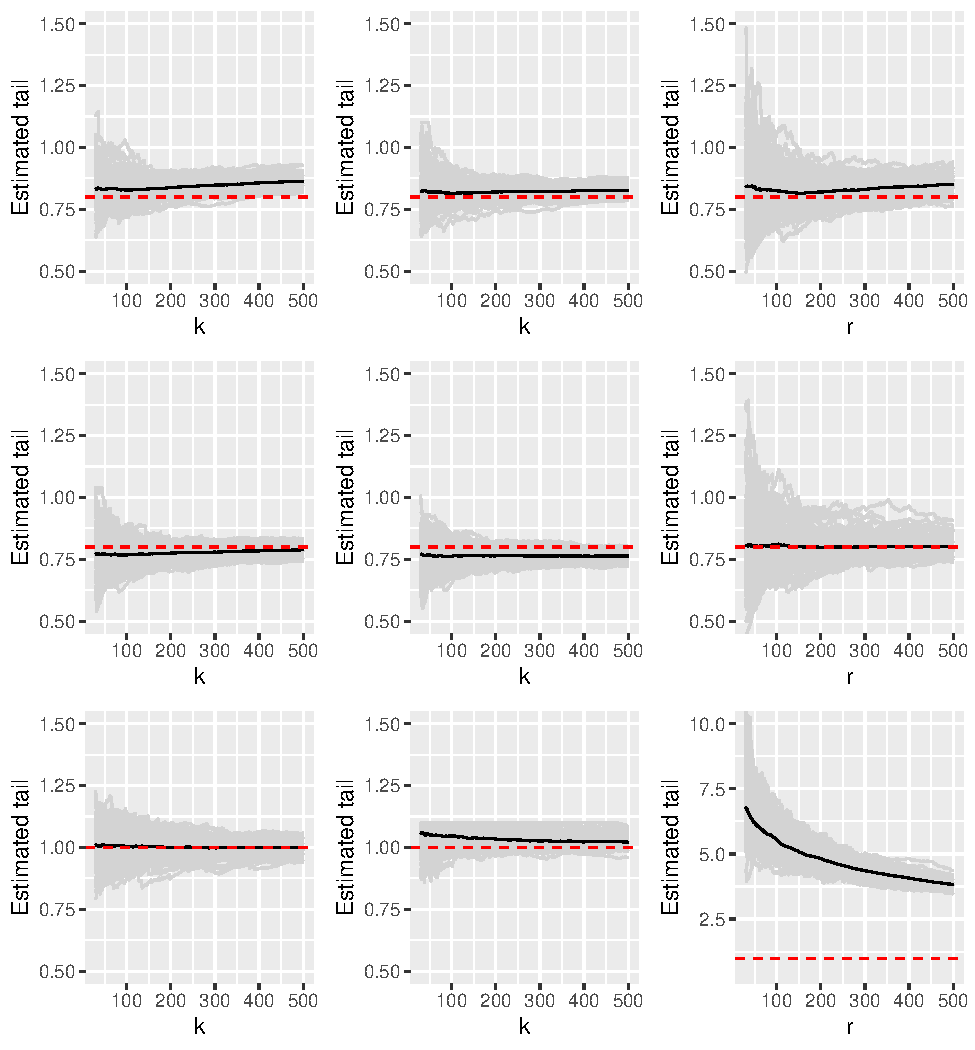
\includegraphics[width=1\linewidth]{article_springer_files/figure-latex/TailSimuplots-1} 

}

\caption{\label{Fig:TailSimu} Stability Plots for m=100 simulation runs for stable distributed waiting times with a tail parameter of 0.8 (top row), Pareto distributed waiting times with tail parameter 0.8 (middle row) and \DIFdelbeginFL \DIFdelFL{exponential }\DIFdelendFL \DIFaddbeginFL \DIFaddFL{exponentially }\DIFaddendFL distributed waiting times (lower row). Left column: log-moment estimator, middle column: MLE, right column: Hill estimator. The grey thin lines are the stability plots for the different simulation runs and the dark lines are their means. The red dotted line shows the true tail parameter. }\label{fig:TailSimuplots}
\end{figure}

\begin{figure}

{\centering 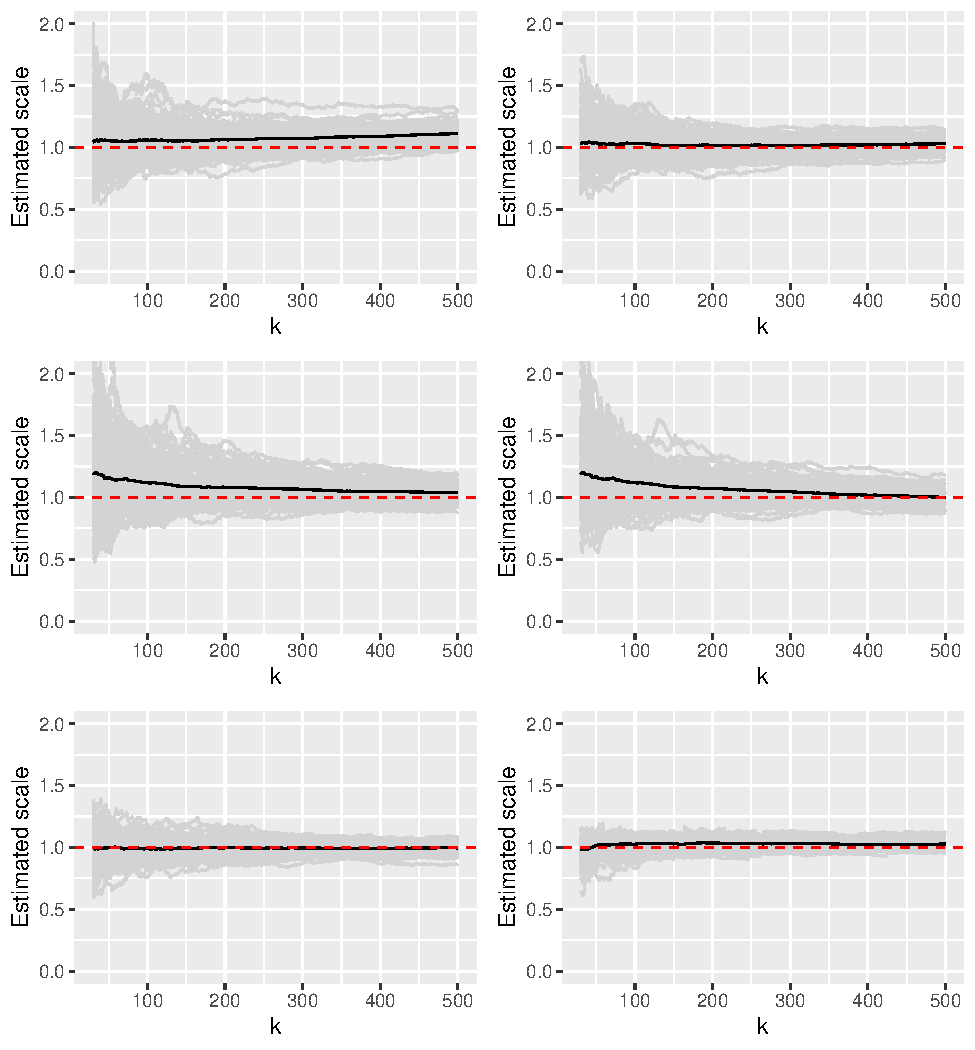
\includegraphics[width=0.9\linewidth]{article_springer_files/figure-latex/ScaleSimuplots-1} 

}

\caption{\label{Fig:ScaleSimu} Stability Plots for m=100 simulation runs for stable distributed waiting times with a tail parameter of 0.8 (top row), Pareto distributed waiting times with tail parameter 0.8 (middle row) and \DIFdelbeginFL \DIFdelFL{exponential }\DIFdelendFL \DIFaddbeginFL \DIFaddFL{exponentially }\DIFaddendFL distributed waiting times (lower row). Left column: log-moment estimator, right column: MLE. The grey thin lines are the stability plots for the different simulation runs and the dark lines are their means. The red dotted line shows the true tail parameter.}\label{fig:ScaleSimuplots}
\end{figure}

\hypertarget{data-example}{%
\section{Data example}\label{data-example}}

We now want to apply the proposed method to a real data example, the
solar flare data which was already mentioned in Section 1 and can be
seen in Figure \ref{fig:thresholdedBursty}. The data were extracted from
the ``complete Hard X Ray Burst Spectrometer event list'', a
comprehensive reference for all measurements of the Hard X Ray Burst
Spectrometer on NASA's Solar Maximum Mission from the time of launch on
Feb 14, 1980 to the end of the mission in Dec 1989. 12,772 events were
detected, with the ``vast majority being solar flares''. To assure
stationarity and due to missing values during the years 1983 and 1984,
we based our analysis just on the year 1982, in which 2,488 events
happened. The list includes the start time, peak time, duration, and
peak rate of each event. We have used ``start time'' as the variable for
event times, and ``peak rate'' as the variable for event magnitudes.

Before we apply the POT approach described in Section 5 to the solar
flare data, we first have to check if all model assumptions are
\DIFdelbegin \DIFdel{full-filled}\DIFdelend \DIFaddbegin \DIFadd{fulfilled}\DIFaddend . The CTRE model is based on three main assumptions, which are
repeated below. For each assumption, we suggest one means of checking if
it holds:

\begin{description}
\item[i.i.d.:]
After removing the ``noise observations'' below the smallest threshold
\(\ell_0\), the pair sequence \((T(\ell_0, i), X(\ell_0,i))\) is i.i.d.
An indication if this is true is given by an auto-correlation plot for
the logarithms (to ensure finite moments) of the two time series.
\item[Uncoupled:]
Each \(T(\ell, i)\) is independent of each \(X(\ell, i)\). We propose an
empirical copula plot to check for any dependence.
\item[\({\rm ML}(\beta, \sigma)\) distribution of \(T(\ell, i)\):]
Apply a cutoff at the lowest threshold \(\ell_0\), extract the threshold
crossing times, and create a QQ Plot for the Mittag-Leffler
distribution. Use a log-moment estimate of the tail parameter for the
theoretical / population quantiles of the plot.
\end{description}

Figures \ref{fig:flare-diagnostics-1}, \ref{fig:flare-diagnostics-2} and
\ref{fig:flare-diagnostics-3} show the diagnostic plots for a minimum
threshold chosen at the 200th order statistic. There is some residual
autocorrelation for the sequence of threshold exceedance times that is
not accounted for by the CTRE model.

\begin{figure}
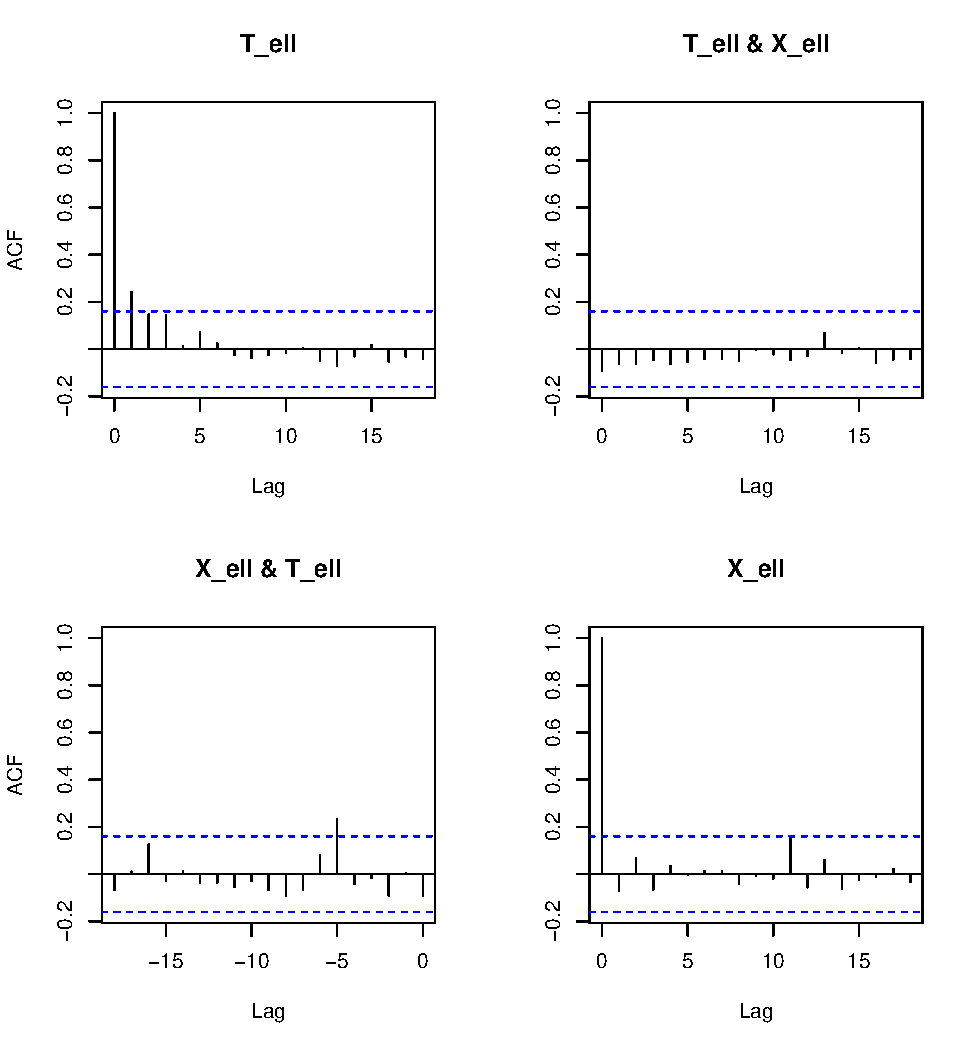
\includegraphics[width=\textwidth]{article_springer_files/figure-latex/flare-diagnostics-1-1} \caption{\label{fig:flare-diagnostics-1} Diagnostic plots for the solar flare data: auto-correlation function.}\label{fig:flare-diagnostics-1}
\end{figure}

\begin{figure}

{\centering 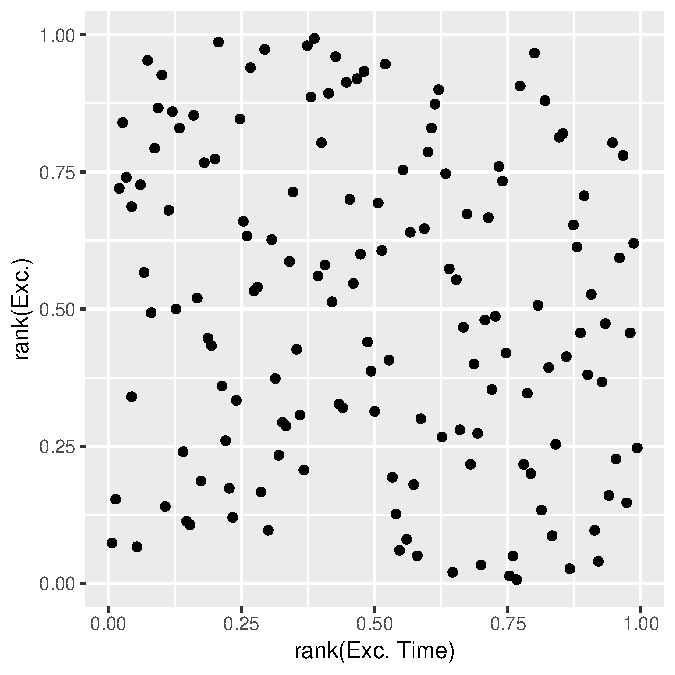
\includegraphics[width=0.7\linewidth]{article_springer_files/figure-latex/flare-diagnostics-2-1} 

}

\caption{\label{fig:flare-diagnostics-2} Diagnostic plots for the solar flare data: empirical copula.}\label{fig:flare-diagnostics-2}
\end{figure}

\begin{figure}

{\centering 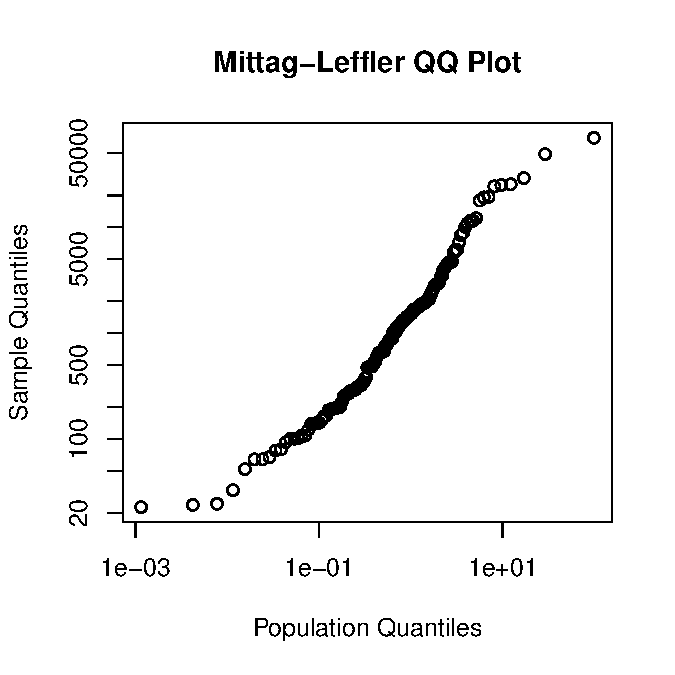
\includegraphics[width=0.7\linewidth]{article_springer_files/figure-latex/flare-diagnostics-3-1} 

}

\caption{\label{fig:flare-diagnostics-3} Diagnostic plots for the solar flare data: QQ Plot.}\label{fig:flare-diagnostics-3}
\end{figure}

Figure \ref{fig:flares} shows the stability plots for the solar flare
data, on the left for the tail parameter and on the right for the scale
parameter. \DIFdelbegin \DIFdel{Dotted lines show }\DIFdelend \DIFaddbegin \DIFadd{The dark grey ranges correspond to }\DIFaddend 95\% confidence intervals,
which are derived from the asymptotic normality of the log-moments
estimators (Cahoy\DIFaddbegin \DIFadd{, }\DIFaddend 2013) and the \(\delta\)-method (Gill and Straka\DIFaddbegin \DIFadd{,
}\DIFaddend 2017)\DIFdelbegin \DIFdel{, }\DIFdelend \DIFaddbegin \DIFadd{; }\DIFaddend dashed lines show the deduced \DIFaddbegin \DIFadd{true }\DIFaddend values of \(\beta\)
resp.~\(\sigma_0\). The stability plot for the tail stabilizes nicely
\DIFdelbegin \DIFdel{round about }\DIFdelend \DIFaddbegin \DIFadd{around }\DIFaddend 0.85 (dashed line), while \DIFdelbegin \DIFdel{it is a little bit harder to deduce an estimate for }\DIFdelend the scale parameter \DIFdelbegin \DIFdel{. Howerever, the stability plot for the scale parameter
seems to stabilize round about }\DIFdelend \DIFaddbegin \DIFadd{stabilizes less
obviously near }\DIFaddend \(3 \times 10^7\) \DIFdelbegin \DIFdel{(dashed line)}\DIFdelend \DIFaddbegin \DIFadd{(dashed line). The growth of the scale
parameter for lower threshold appears to be closer to linear in
\(p_{\ell}\), rather than proportional to \(p_{\ell}^{1/0.85}\) as
suggested by the Mittag-Leffler fits. The reason for this is likely that
the overall goodness of fit as compared to an exponential distribution
is improved due to the peaked shape of the Mittag-Leffler distribution
near \(0\), rather than its tail behaviour at \(\infty\). The reported
fit should hence come with the caveat that a Mittag-Leffler distribution
models exceedance times well only up to certain time-scales. More
research is needed into the modelling of scale transitions, where
inter-exceedance times appear to have different power laws across
different time scales}\DIFaddend .

\begin{figure}
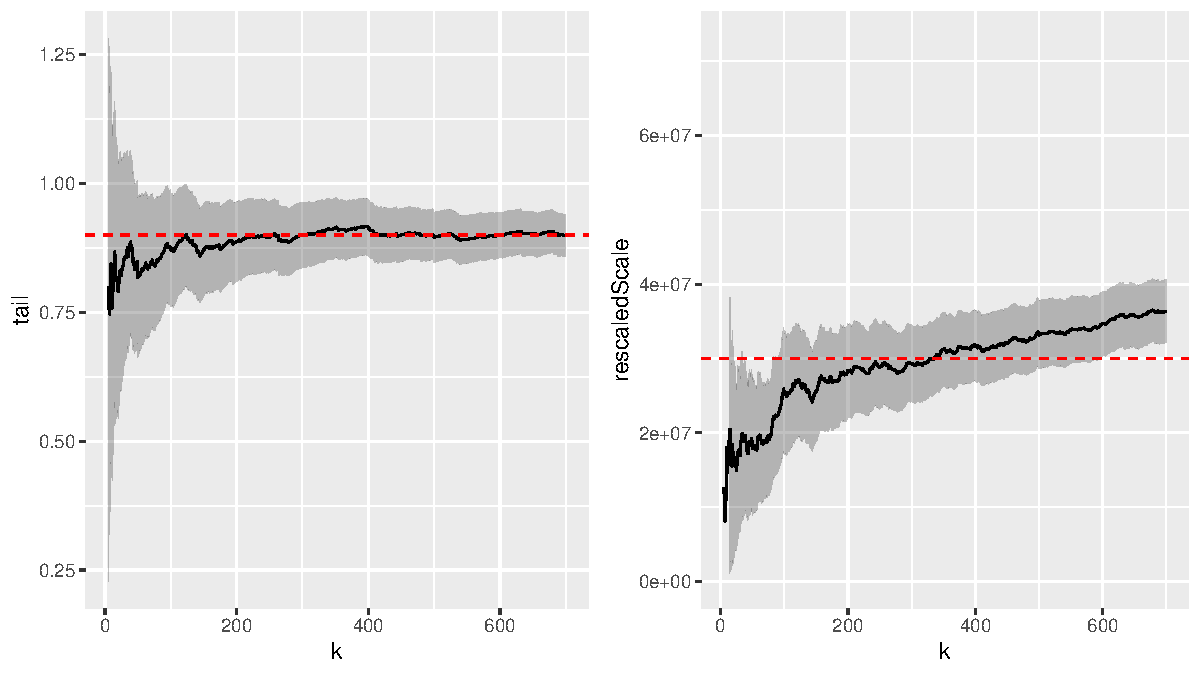
\includegraphics[width=\textwidth]{article_springer_files/figure-latex/solar-flare-tail-scale-1} \caption{\label{fig:flares} Stability plots for the tail and scale parameter of the Mittag-Leffler distribution of the Solar Flare dataset. Dotted horizontal lines are at $\beta = 0.85$ and $\sigma_0 = 3 \times 10^7$ seconds $\approx 0.95$ years.}\label{fig:solar-flare-tail-scale}
\end{figure}

The fit with a Mittag-Leffler distribution (\(\beta = 0.85\)) is good
(see Figure \ref{fig:flare-diagnostics-3}), though there are signs that
the power-law tail tapers off for very large inter-threshold crossing
times. There is no apparent dependence between threshold exceedance
times and event magnitudes seen in the copula plot (see Figure
\ref{fig:flare-diagnostics-2}). We also counduct a bootstrapped LRT for
the null hypothesis of \DIFdelbegin \DIFdel{exponential }\DIFdelend \DIFaddbegin \DIFadd{exponentially }\DIFaddend distributed inter-arrival times and
received a \(p\)-value of \(p<0.01\).

\hypertarget{predicting-the-time-of-the-next-threshold-crossing}{%
\section{Predicting the time of the next threshold
crossing}\label{predicting-the-time-of-the-next-threshold-crossing}}

According to Figure \ref{fig:flares}, for a threshold \(\ell\) at the
\(k\)-th order statistic, the \DIFdelbegin \DIFdel{fitted }\DIFdelend \DIFaddbegin \DIFadd{estimated }\DIFaddend threshold exceedance time
distribution is \[
T(\ell) \sim {\rm ML}(\beta, k^{-1/\beta} \sigma_0), 
\] where \(\beta = 0.85\) and \(\sigma_0 = 3.0 \times 10^7 {\rm sec}\).
Unlike the exponential distribution, the Mittag-Leffler distribution is
not memoryless, and the probability density of the time \(t\) until the
next threshold crossing will depend on the time \(t_0\) elapsed since
the last threshold crossing. This density \DIFdelbegin \DIFdel{equals }\DIFdelend \DIFaddbegin \DIFadd{is approximately equal to }\DIFaddend \[
p(t|\beta, \sigma_0, \ell, t_0) \DIFdelbegin \DIFdel{= }\DIFdelend \DIFaddbegin \DIFadd{\approx }\DIFaddend \frac{f(t + t_0 | \beta, k^{-1/\beta} \sigma_0)}{\mathbf P[T_\ell > t_0]}
\] where \(f(\,\cdot\, | \beta, k^{-1/\beta} \sigma_0)\) is the
probability density of \({\rm ML}(\beta, k^{-1/\beta} \sigma_0)\). The
more time has passed without a threshold crossing, the more the
probability distribution shifts towards larger values for the next
crossing (see Figure \ref{fig:hazard}, left panel). The hazard rate \[
h(t) = \frac{f(t| \beta, k^{-1/\beta} \sigma_0))}{\int_t^\infty f(\tau| \beta, k^{-1/\beta} \sigma_0))\,d\tau}
\] represents the risk of a threshold crossing per unit time, and is a
decreasing function for the Mittag-Leffler distribution.

\begin{figure}
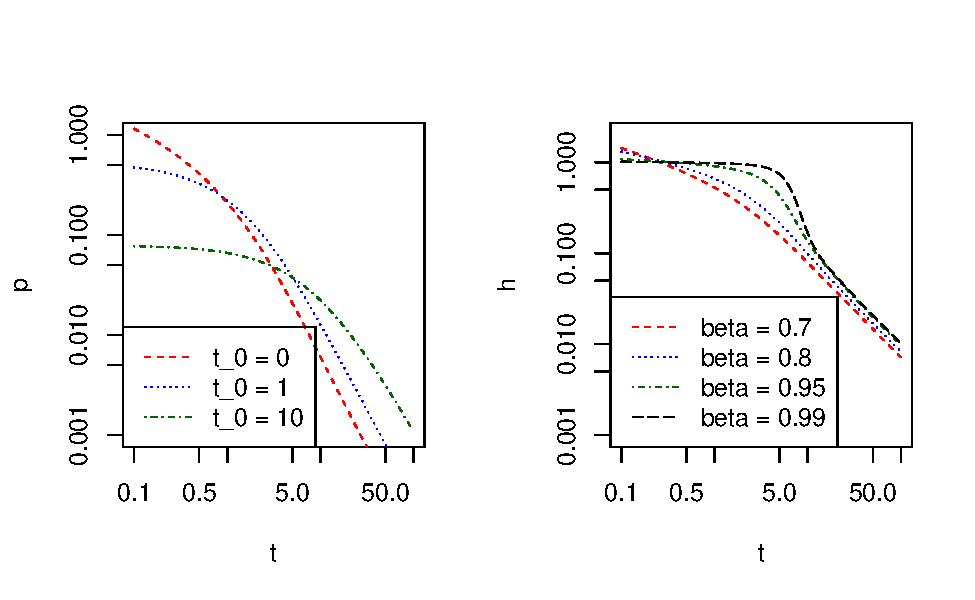
\includegraphics[width=\textwidth]{article_springer_files/figure-latex/hazard-1} \caption{\label{fig:hazard} Left: Conditional distribution of time until next threshold crossing, depending on elapsed time $t_0$ since last crossing ($\beta = 0.8$, $\sigma_0 = 1$). Right: Hazard rate depending on tail parameter $\beta$.}\label{fig:hazard}
\end{figure}

The closer \(\beta\) is to \(1\), the more the hazard rate mimics that
of an exponential distribution (a constant function, see Figure
\ref{fig:hazard}, right panel).

\hypertarget{discussion-conclusion}{%
\section{Discussion \& Conclusion}\label{discussion-conclusion}}

We have extended the POT (Peaks-over-Threshold) model, a mainstay of
extreme value theory, to ``bursty'' time series, which have been studied
intensively in statistical physics. Burstiness is characterized by
power-law waiting times between events, and we have shown that the
Mittag-Leffler distribution arises naturally as a scaling limit for the
inter-exceedance times of high thresholds. Moreover, we have derived the
following non-linear scaling behaviour:
\DIFdelbegin \DIFdel{\(\sigma \sim p^{-1/\beta}\)}\DIFdelend \DIFaddbegin \DIFadd{\(\sigma \sim p_{\ell}^{-1/\beta}\)}\DIFaddend , where \(\sigma\) is the scale
parameter of the distribution of threshold exceedance times,
\DIFdelbegin \DIFdel{\(p\) }\DIFdelend \DIFaddbegin \DIFadd{\(p_{\ell}\) }\DIFaddend is the fraction of magnitudes above the threshold, and
\(\beta\) the exponent of the power law. This ``anomalous'' scaling
behaviour in the bursty setting entails two phenomena:

\begin{enumerate}
\def\labelenumi{\roman{enumi})}
\item
  a heavy tail of the inter-arrival time distribution of threshold
  crossings (long rests), and
\item
  a high propensity for more threshold crossing events immediately after
  each threshold crossing event (bursts).
\end{enumerate}

The Mittag-Leffler distribution captures both phenomena, due to its
heavy tail as well as its stretched exponential (peaked) asymptotics for
small times. It generalizes the exponential distribution, and in the
solar flare data example, this generalization is warranted, because the
likelihood-ratio test is strongly significant.

When we introduced the CTRE model, we assumed that all events are i.i.d.
This assumption is likely sufficient but not necessary for our limit
theorem to hold. Moreover, any data below a (minimum) threshold
\(\ell_0\) is discarded for CTREs, and hence need not satisfy the i.i.d.
assumption. For the purposes of statistical inference, we merely require
that the inter-threshold-crossing times are i.i.d.

The bursty CTRE approach to model ``non-Poissonian'' threshold crossing
times should be contrasted with the (now standard) approach of clusters
of extremes, see e.g.~Ferro and Segers (2003). In this approach, i.i.d.
event sequences of magnitudes are generalized to stationary sequences of
event magnitudes (subject to a mixing condition). The two approaches are
fundamentally different: A clustering model assumes that each event
belongs to one particular (latent) group of events. For bursts, however,
the aim is to identify an underlying scale-free pattern in the event
dynamics, which is often characteristic of complex systems. It is an
interesting open problem to develop quality criteria, based e.g.~on
measures of surprise (Lee \DIFdelbegin \DIFdel{, Fan, and Sisson }\DIFdelend \DIFaddbegin \DIFadd{et al., }\DIFaddend 2015), which guide an applied
statistician in the choice between a clustering and a CTRE approach for
a particular problem. Moreover, we believe it may be possible to unify
the two approaches by considering CTREs based on MRPs with a
\emph{stationary}, rather than i.i.d., sequence of magnitudes.

Finally, a purely scale-free pattern for event times may be too rigid as
an assumption for some bursty time series, because often the
heavy-tailed character of the inter-arrival time distribution does not
hold at all time scales; rather, it applies at short and intermediate
time scales, and is truncated (or tempered, reverting to an exponential
distribution) at very long time scales (see e.g.~\DIFdelbegin \DIFdel{Mark M. Meerschaert ,
Roy, and Shao }\DIFdelend \DIFaddbegin \DIFadd{Meerschaert et al.,
}\DIFaddend 2012; and Aban \DIFdelbegin \DIFdel{, Meerschaert, and Panorska }\DIFdelend \DIFaddbegin \DIFadd{et al., }\DIFaddend 2006). In such situations, a ``tempered''
Mittag-Leffler distribution may provide a more realistic fit, which we
aim to introduce in follow-up work.

\hypertarget{acknowledgements}{%
\section*{Acknowledgements}\label{acknowledgements}}
\addcontentsline{toc}{section}{Acknowledgements}

The authors would like to thank Prof.~Peter Scheffler for insights on
stochastic process limits for CTRMs, Prof.~Roland Fried for discussion
\DIFdelbegin \DIFdel{according }\DIFdelend \DIFaddbegin \DIFadd{regarding }\DIFaddend the statistical methods and Gurtek Gill who helped create the
MittagLeffleR R-package.

\newpage

\hypertarget{references}{%
\section*{References}\label{references}}
\addcontentsline{toc}{section}{References}

\hypertarget{refs}{}
\leavevmode\hypertarget{ref-Aban06}{}%
Aban, \DIFdelbegin \DIFdel{Inmaculada B}\DIFdelend \DIFaddbegin \DIFadd{I.B., Meerschaert}\DIFaddend , \DIFdelbegin \DIFdel{Mark M Meerschaert, and Anna K Panorska. }\DIFdelend \DIFaddbegin \DIFadd{M.M., Panorska, A.K., }\DIFaddend 2006. \DIFdelbegin \DIFdel{``Parameter
Estimation for the Truncated Pareto Distribution. '' }\emph{\DIFdel{J.
Am. Stat. Assoc.}} %DIFAUXCMD
\DIFdelend \DIFaddbegin \DIFadd{Parameter
estimation for the truncated pareto distribution. J. Am. Stat. Assoc.
}\DIFaddend 101\DIFdelbegin \DIFdel{(473): 270--77. }%DIFDELCMD < \url{https://doi.org/10.1198/016214505000000411}%%%
\DIFdel{. }\DIFdelend \DIFaddbegin \DIFadd{, 270--277.
doi:}\href{https://doi.org/10.1198/016214505000000411}{10.1198/016214505000000411}
\DIFaddend 

\leavevmode\hypertarget{ref-Anderson1987}{}%
Anderson, \DIFdelbegin \DIFdel{Kevin K.}\DIFdelend \DIFaddbegin \DIFadd{K.K., }\DIFaddend 1987. \DIFdelbegin \DIFdel{``}\DIFdelend Limit Theorems for General Shock Models with
Infinite Mean Intershock Times. \DIFdelbegin \DIFdel{'' }\emph{\DIFdel{J. Appl. Probab.}} %DIFAUXCMD
\DIFdelend \DIFaddbegin \DIFadd{J. Appl. Probab. }\DIFaddend 24\DIFdelbegin \DIFdel{(2):
449--56. }%DIFDELCMD < \url{http://www.jstor.org/stable/3214268}%%%
\DIFdel{. }\DIFdelend \DIFaddbegin \DIFadd{, 449--456.
}\DIFaddend 

\leavevmode\hypertarget{ref-Bagrow2013}{}%
Bagrow, \DIFdelbegin \DIFdel{James }\DIFdelend \DIFaddbegin \DIFadd{J.}\DIFaddend P., \DIFdelbegin \DIFdel{and Dirk Brockmann. }\DIFdelend \DIFaddbegin \DIFadd{Brockmann, D., }\DIFaddend 2013. \DIFdelbegin \DIFdel{``}\DIFdelend Natural emergence of clusters and
bursts in network evolution. \DIFdelbegin \DIFdel{'' }\emph{\DIFdel{Phys. Rev. X}} %DIFAUXCMD
\DIFdelend \DIFaddbegin \DIFadd{Phys. Rev. X }\DIFaddend 3\DIFdelbegin \DIFdel{(2):
}\DIFdelend \DIFaddbegin \DIFadd{, }\DIFaddend 1--6.
\DIFdelbegin %DIFDELCMD < \url{https://doi.org/10.1103/PhysRevX.3.021016}%%%
\DIFdel{.
}\DIFdelend \DIFaddbegin \DIFadd{doi:}\href{https://doi.org/10.1103/PhysRevX.3.021016}{10.1103/PhysRevX.3.021016}
\DIFaddend 

\leavevmode\hypertarget{ref-Barabasi2005}{}%
Barabási, \DIFdelbegin \DIFdel{Albert László.}\DIFdelend \DIFaddbegin \DIFadd{A.L., }\DIFaddend 2005. \DIFdelbegin \DIFdel{``}\DIFdelend The origin of bursts and heavy tails in human
dynamics. \DIFdelbegin \DIFdel{'' }\emph{\DIFdel{Nature}} %DIFAUXCMD
\DIFdelend \DIFaddbegin \DIFadd{Nature }\DIFaddend 435\DIFdelbegin \DIFdel{(May): 207--11.
}%DIFDELCMD < \url{https://doi.org/10.1038/nature03459}%%%
\DIFdel{.
}\DIFdelend \DIFaddbegin \DIFadd{, 207--211.
doi:}\href{https://doi.org/10.1038/nature03459}{10.1038/nature03459}
\DIFaddend 

\leavevmode\hypertarget{ref-Basrak2014}{}%
Basrak, \DIFdelbegin \DIFdel{Bojan, and Drago }\DIFdelend \DIFaddbegin \DIFadd{B., }\DIFaddend Špoljarić\DIFdelbegin \DIFdel{. }\DIFdelend \DIFaddbegin \DIFadd{, D., }\DIFaddend 2015. \DIFdelbegin \DIFdel{``}\DIFdelend Extremes of random variables observed
in renewal times. \DIFdelbegin \DIFdel{'' }\emph{\DIFdel{Stat. Probab. Lett.}} %DIFAUXCMD
\DIFdelend \DIFaddbegin \DIFadd{Stat. Probab. Lett. }\DIFaddend 97\DIFdelbegin \DIFdel{: 216--21. }%DIFDELCMD < \url{https://doi.org/10.1016/j.spl.2014.11.025}%%%
\DIFdel{. }\DIFdelend \DIFaddbegin \DIFadd{, 216--221.
doi:}\href{https://doi.org/10.1016/j.spl.2014.11.025}{10.1016/j.spl.2014.11.025}
\DIFaddend 

\leavevmode\hypertarget{ref-beirlantBook}{}%
Beirlant, \DIFdelbegin \DIFdel{Jan, Yuri Goegebeur, Johan Segers, and Jozef Teugels. }\DIFdelend \DIFaddbegin \DIFadd{J., Goegebeur, Y., Segers, J., Teugels, J., }\DIFaddend 2006. \DIFdelbegin \emph{\DIFdel{Statistics of extremes: theory and applications}}%DIFAUXCMD
\DIFdelend \DIFaddbegin \DIFadd{Statistics
of extremes: theory and applications}\DIFaddend . John Wiley \& Sons.

\leavevmode\hypertarget{ref-Benson2007}{}%
Benson, \DIFdelbegin \DIFdel{David A}\DIFdelend \DIFaddbegin \DIFadd{D.A., Schumer}\DIFaddend , \DIFdelbegin \DIFdel{Rina Schumer, and Mark M Meerschaert. }\DIFdelend \DIFaddbegin \DIFadd{R., Meerschaert, M.M., }\DIFaddend 2007. \DIFdelbegin \DIFdel{``}\DIFdelend Recurrence of
extreme events with power-law interarrival times. \DIFdelbegin \DIFdel{''
}\emph{\DIFdel{Geophys. Res. Lett.}} %DIFAUXCMD
\DIFdelend \DIFaddbegin \DIFadd{Geophys. Res. Lett.
}\DIFaddend 34\DIFdelbegin \DIFdel{(l16404): }\DIFdelend \DIFaddbegin \DIFadd{, }\DIFaddend DOI:10.1029/2007GL030767.
\DIFdelbegin %DIFDELCMD < \url{https://doi.org/10.1029/2007GL030767}%%%
\DIFdel{.}\DIFdelend \DIFaddbegin \DIFadd{doi:}\href{https://doi.org/10.1029/2007GL030767}{10.1029/2007GL030767}
\DIFaddend 

\leavevmode\DIFaddbegin \hypertarget{ref-BinghamGoldieTeugels}{}%DIF > 
\DIFadd{Bingham, N.H., Goldie, C.M., Teugels, J.L., 1989. Regular variation.
Cambridge university press.
}

\leavevmode\DIFaddend \hypertarget{ref-Cahoy2013}{}%
Cahoy, \DIFdelbegin \DIFdel{Dexter O.}\DIFdelend \DIFaddbegin \DIFadd{D.O., }\DIFaddend 2013. \DIFdelbegin \DIFdel{``}\DIFdelend Estimation of Mittag-Leffler Parameters. \DIFdelbegin \DIFdel{''
}\emph{\DIFdel{Commun. Stat. - Simul. Comput.}} %DIFAUXCMD
\DIFdelend \DIFaddbegin \DIFadd{Commun.
Stat. - Simul. Comput. }\DIFaddend 42\DIFdelbegin \DIFdel{(2): 303--15.
}%DIFDELCMD < \url{https://doi.org/10.1080/03610918.2011.640094}%%%
\DIFdel{. }\DIFdelend \DIFaddbegin \DIFadd{, 303--315.
doi:}\href{https://doi.org/10.1080/03610918.2011.640094}{10.1080/03610918.2011.640094}
\DIFaddend 

\leavevmode\hypertarget{ref-Cahoy2010}{}%
Cahoy, \DIFdelbegin \DIFdel{Dexter O, Vladimir V.Uchaikin, and Wojbor A.Woyczynski}\DIFdelend \DIFaddbegin \DIFadd{D.O}\DIFaddend .\DIFaddbegin \DIFadd{, Uchaikin, V.V., Woyczynski, W.A., }\DIFaddend 2010. \DIFdelbegin \DIFdel{``}\DIFdelend Parameter
estimation for fractional Poisson processes. \DIFdelbegin \DIFdel{'' }\emph{\DIFdel{J.
Stat. Plan. Inference}} %DIFAUXCMD
\DIFdelend \DIFaddbegin \DIFadd{J. Stat. Plan. Inference
}\DIFaddend 140\DIFdelbegin \DIFdel{(11): 3106--20. }%DIFDELCMD < \url{https://doi.org/10.1016/j.jspi.2010.04.016}%%%
\DIFdel{. }\DIFdelend \DIFaddbegin \DIFadd{, 3106--3120.
doi:}\href{https://doi.org/10.1016/j.jspi.2010.04.016}{10.1016/j.jspi.2010.04.016}
\DIFaddend 

\leavevmode\hypertarget{ref-ColesBook}{}%
Coles, S.\DIFaddbegin \DIFadd{, }\DIFaddend 2001. \DIFdelbegin \emph{\DIFdel{An Introduction to Statistical Modelling of
Extreme Values}}%DIFAUXCMD
\DIFdel{. London: }\DIFdelend \DIFaddbegin \DIFadd{An Introduction to Statistical Modelling of Extreme
Values. }\DIFaddend Springer-Verlag\DIFaddbegin \DIFadd{, London}\DIFaddend .

\leavevmode\hypertarget{ref-davison1997bootstrap}{}%
Davison, \DIFdelbegin \DIFdel{Anthony Christopher, David Victor Hinkley, and others.}\DIFdelend \DIFaddbegin \DIFadd{A.C., Hinkley, D.V., others, }\DIFaddend 1997. \DIFdelbegin \emph{\DIFdel{Bootstrap Methods and Their Application}}%DIFAUXCMD
\DIFdel{. Vol. 1. }\DIFdelend \DIFaddbegin \DIFadd{Bootstrap methods and their
application. }\DIFaddend Cambridge university press.

\leavevmode\hypertarget{ref-HXRBS}{}%
Dennis, \DIFdelbegin \DIFdel{Brian R}\DIFdelend \DIFaddbegin \DIFadd{B.R., Orwig, L.E., Kennard, G.S., Labow, G.J., Schwartz, R.A.,
Shaver, A.R., Tolbert, A.K.}\DIFaddend , \DIFdelbegin \DIFdel{L E Orwig, G S Kennard, G J Labow, R A Schwartz,
A R
Shaver, and AK Tolbert.}\DIFdelend 1991. \DIFdelbegin \DIFdel{``}\DIFdelend The complete Hard X Ray Burst
Spectrometer event list, 1980-1989.
\DIFdelbegin \DIFdel{''
}%DIFDELCMD < \url{https://umbra.nascom.nasa.gov/smm/hxrbs.html}%%%
\DIFdel{.
}\DIFdelend 

\leavevmode\hypertarget{ref-Esary1973}{}%
Esary, J.D., \DIFdelbegin \DIFdel{and }\DIFdelend \DIFaddbegin \DIFadd{Marshall, }\DIFaddend A.W.\DIFdelbegin \DIFdel{Marshall. }\DIFdelend \DIFaddbegin \DIFadd{, }\DIFaddend 1973. \DIFdelbegin \DIFdel{``}\DIFdelend Shock Models and Wear Processes.
\DIFdelbegin \DIFdel{'' }%DIFDELCMD < \url{https://doi.org/10.1214/aop/1176996891}%%%
\DIFdel{.
}\DIFdelend \DIFaddbegin \DIFadd{doi:}\href{https://doi.org/10.1214/aop/1176996891}{10.1214/aop/1176996891}
\DIFaddend 

\leavevmode\hypertarget{ref-ferro2003inference}{}%
Ferro, \DIFdelbegin \DIFdel{Christopher AT, and Johan Segers. }\DIFdelend \DIFaddbegin \DIFadd{C.A., Segers, J., }\DIFaddend 2003. \DIFdelbegin \DIFdel{``Inference for Clusters
of Extreme Values.
'' }\emph{\DIFdel{Journal of the Royal Statistical Society:
Series B (Statistical Methodology)}} %DIFAUXCMD
\DIFdel{65 (2) : 545--56}\DIFdelend \DIFaddbegin \DIFadd{Inference for clusters of extreme values.
Journal of the Royal Statistical Society: Series B (Statistical
Methodology) 65, 545--556}\DIFaddend .

\leavevmode\hypertarget{ref-MittagLeffleR}{}%
Gill, \DIFdelbegin \DIFdel{Gurtek, and Peter Straka. }\DIFdelend \DIFaddbegin \DIFadd{G., Straka, P., }\DIFaddend 2017. \DIFdelbegin \emph{\DIFdel{MittagLeffleR: Using the
Mittag-Leffler Distributions in R}}%DIFAUXCMD
\DIFdel{.
}%DIFDELCMD < \url{https://strakaps.github.io/MittagLeffleR/}%%%
\DIFdel{.
}\DIFdelend \DIFaddbegin \DIFadd{MittagLeffleR: Using the mittag-leffler
distributions in r.
}\DIFaddend 

\leavevmode\hypertarget{ref-Gut1999}{}%
Gut, \DIFdelbegin \DIFdel{Allan, and Jürg }\DIFdelend \DIFaddbegin \DIFadd{A., }\DIFaddend Hüsler\DIFdelbegin \DIFdel{. }\DIFdelend \DIFaddbegin \DIFadd{, J., }\DIFaddend 1999. \DIFdelbegin \DIFdel{``}\DIFdelend Extreme Shock Models. \DIFdelbegin \DIFdel{''
}\emph{\DIFdel{Extremes}}%DIFAUXCMD
\DIFdel{, no. 1983: }\DIFdelend \DIFaddbegin \DIFadd{Extremes }\DIFaddend 295--307.
\DIFdelbegin %DIFDELCMD < \url{http://link.springer.com/article/10.1023/A:1009959004020}%%%
\DIFdel{.
}\DIFdelend 

\leavevmode\hypertarget{ref-Haubold11}{}%
Haubold, H.J., \DIFaddbegin \DIFadd{Mathai, }\DIFaddend A.M.\DIFdelbegin \DIFdel{Mathai, and }\DIFdelend \DIFaddbegin \DIFadd{, Saxena, }\DIFaddend R.K.\DIFdelbegin \DIFdel{Saxena. }\DIFdelend \DIFaddbegin \DIFadd{, }\DIFaddend 2011. \DIFdelbegin \DIFdel{``}\DIFdelend Mittag-Leffler
Functions and Their Applications. \DIFdelbegin \DIFdel{'' }\emph{\DIFdel{J. Appl. Math.}} %DIFAUXCMD
\DIFdelend \DIFaddbegin \DIFadd{J. Appl. Math. }\DIFaddend 2011\DIFdelbegin \DIFdel{: }\DIFdelend \DIFaddbegin \DIFadd{, }\DIFaddend 1--51.
\DIFdelbegin %DIFDELCMD < \url{https://doi.org/10.1155/2011/298628}%%%
\DIFdel{.
}\DIFdelend \DIFaddbegin \DIFadd{doi:}\href{https://doi.org/10.1155/2011/298628}{10.1155/2011/298628}
\DIFaddend 

\leavevmode\hypertarget{ref-hawkes1971point}{}%
Hawkes, \DIFdelbegin \DIFdel{Alan G.}\DIFdelend \DIFaddbegin \DIFadd{A.G., }\DIFaddend 1971. \DIFdelbegin \DIFdel{``}\DIFdelend Point spectra of some mutually exciting point
processes. \DIFdelbegin \DIFdel{'' }\emph{\DIFdel{J. R. Stat. Soc. Ser. B Stat. Methodol.}}%DIFAUXCMD
\DIFdel{, 438--43. }\DIFdelend \DIFaddbegin \DIFadd{J. R. Stat. Soc. Ser. B Stat. Methodol. 438--443.
}\DIFaddend 

\leavevmode\DIFdelbegin %DIFDELCMD < \hypertarget{ref-hees2017coupled}{}%%%
\DIFdelend \DIFaddbegin \hypertarget{ref-hees2016joint}{}\DIFaddend %
Hees, \DIFdelbegin \DIFdel{Katharina, and Hans-Peter Scheffler. }\DIFdelend \DIFaddbegin \DIFadd{K., Scheffler, H.-P., }\DIFaddend 2018a. \DIFdelbegin \DIFdel{``Coupled Continuous
Time Random Maxima. '' }\emph{\DIFdel{Extremes}} %DIFAUXCMD
\DIFdel{21 (2).
}\DIFdelend \DIFaddbegin \DIFadd{On joint sum/max stability and
sum/max domains of attraction. Probability and Mathematical Statistics
38.
}\DIFaddend 

\leavevmode\DIFdelbegin %DIFDELCMD < \hypertarget{ref-hees2016joint}{}%%%
\DIFdelend \DIFaddbegin \hypertarget{ref-hees2017coupled}{}\DIFaddend %
\DIFdelbegin \DIFdel{---------.}\DIFdelend \DIFaddbegin \DIFadd{Hees, K., Scheffler, H.-P., }\DIFaddend 2018b. \DIFdelbegin \DIFdel{``On Joint Sum/Max Stability and Sum/Max Domains of
Attraction. '' }\emph{\DIFdel{Probability and Mathematical Statistics}} %DIFAUXCMD
\DIFdel{38 (1).}\DIFdelend \DIFaddbegin \DIFadd{Coupled continuous time random
maxima. Extremes 21.
}\DIFaddend 

\leavevmode\DIFaddbegin \hypertarget{ref-CTRE}{}%DIF > 
\DIFadd{Hees, K., Straka, P., 2018. CTRE: Thresholding bursty time series.
doi:}\href{https://doi.org/10.6084/m9.figshare.6243434.v2}{10.6084/m9.figshare.6243434.v2}

\leavevmode\DIFaddend \hypertarget{ref-hill1975simple}{}%
Hill, \DIFdelbegin \DIFdel{Bruce M.1975. ``A Simple General Approach to Inference About the Tail of a Distribution. '' }\emph{\DIFdel{The Annals of Statistics}}%DIFAUXCMD
\DIFdelend \DIFaddbegin \DIFadd{B.M.}\DIFaddend , \DIFdelbegin \DIFdel{1163--74}\DIFdelend \DIFaddbegin \DIFadd{1975. A simple general approach to inference about the tail
of a distribution. The annals of statistics 1163--1174}\DIFaddend .

\leavevmode\hypertarget{ref-Karsai2012}{}%
Karsai, \DIFdelbegin \DIFdel{Márton, Kimmo Kaski, Albert László }\DIFdelend \DIFaddbegin \DIFadd{M., Kaski, K., }\DIFaddend Barabási, \DIFdelbegin \DIFdel{and János }\DIFdelend \DIFaddbegin \DIFadd{A.L., }\DIFaddend Kertész\DIFdelbegin \DIFdel{.
}\DIFdelend \DIFaddbegin \DIFadd{, J., }\DIFaddend 2012. \DIFdelbegin \DIFdel{``}\DIFdelend Universal
features of correlated bursty behaviour. \DIFdelbegin \DIFdel{'' }\emph{\DIFdel{Sci.
Rep.}} %DIFAUXCMD
\DIFdelend \DIFaddbegin \DIFadd{Sci. Rep. }\DIFaddend 2.
\DIFdelbegin %DIFDELCMD < \url{https://doi.org/10.1038/srep00397}%%%
\DIFdel{. }\DIFdelend \DIFaddbegin \DIFadd{doi:}\href{https://doi.org/10.1038/srep00397}{10.1038/srep00397}
\DIFaddend 

\leavevmode\hypertarget{ref-Karsai2011}{}%
Karsai, \DIFdelbegin \DIFdel{Márton, M.}\DIFdelend \DIFaddbegin \DIFadd{M., }\DIFaddend Kivelä, \DIFaddbegin \DIFadd{M., Pan, }\DIFaddend R.K.\DIFdelbegin \DIFdel{Pan, K. Kaski, J. Kertész, Albert
László }\DIFdelend \DIFaddbegin \DIFadd{, Kaski, K., Kertész, J., }\DIFaddend Barabási,
\DIFdelbegin \DIFdel{and J.}\DIFdelend \DIFaddbegin \DIFadd{A.L., }\DIFaddend Saramäki\DIFdelbegin \DIFdel{. }\DIFdelend \DIFaddbegin \DIFadd{, J., }\DIFaddend 2011. \DIFdelbegin \DIFdel{``}\DIFdelend Small but slow world: How network topology and
burstiness slow down spreading. \DIFdelbegin \DIFdel{'' }\emph{\DIFdel{Phys. Rev.
E - Stat. Nonlinear, Soft Matter Phys.}} %DIFAUXCMD
\DIFdelend \DIFaddbegin \DIFadd{Phys. Rev. E - Stat. Nonlinear, Soft
Matter Phys. }\DIFaddend 83\DIFdelbegin \DIFdel{: }\DIFdelend \DIFaddbegin \DIFadd{, }\DIFaddend 1--4.
\DIFdelbegin %DIFDELCMD < \url{https://doi.org/10.1103/PhysRevE.83.025102}%%%
\DIFdel{.
}\DIFdelend \DIFaddbegin \DIFadd{doi:}\href{https://doi.org/10.1103/PhysRevE.83.025102}{10.1103/PhysRevE.83.025102}
\DIFaddend 

\leavevmode\hypertarget{ref-kozubowski2001}{}%
Kozubowski, \DIFdelbegin \DIFdel{Tomasz J.}\DIFdelend \DIFaddbegin \DIFadd{T.J., }\DIFaddend 2001. \DIFdelbegin \DIFdel{``Fractional Moment Estimation of Linnik and
Mittag-Leffler Parameters. '' }\emph{\DIFdel{Mathematical and Computer Modelling}}
%DIFAUXCMD
\DIFdelend \DIFaddbegin \DIFadd{Fractional moment estimation of linnik and
mittag-leffler parameters. Mathematical and computer modelling }\DIFaddend 34\DIFdelbegin \DIFdel{(9-11): 1023--35}\DIFdelend \DIFaddbegin \DIFadd{,
1023--1035}\DIFaddend .

\leavevmode\hypertarget{ref-Laskin2003}{}%
Laskin, \DIFdelbegin \DIFdel{Nick.}\DIFdelend \DIFaddbegin \DIFadd{N., }\DIFaddend 2003. \DIFdelbegin \DIFdel{``}\DIFdelend Fractional Poisson process. \DIFdelbegin \DIFdel{'' }\emph{\DIFdel{Commun.
Nonlinear Sci. Numer. Simul.}} %DIFAUXCMD
\DIFdelend \DIFaddbegin \DIFadd{Commun. Nonlinear Sci.
Numer. Simul. }\DIFaddend 8\DIFdelbegin \DIFdel{(3-4): 201--13. }%DIFDELCMD < \url{https://doi.org/10.1016/S1007-5704(03)00037-6}%%%
\DIFdel{.
}\DIFdelend \DIFaddbegin \DIFadd{, 201--213.
doi:}\href{https://doi.org/10.1016/S1007-5704(03)00037-6}{10.1016/S1007-5704(03)00037-6}
\DIFaddend 

\leavevmode\hypertarget{ref-Lee15}{}%
Lee, J., \DIFdelbegin \DIFdel{Y. Fan, and }\DIFdelend \DIFaddbegin \DIFadd{Fan, Y., Sisson, }\DIFaddend S.A.\DIFdelbegin \DIFdel{Sisson. }\DIFdelend \DIFaddbegin \DIFadd{, }\DIFaddend 2015. \DIFdelbegin \DIFdel{``}\DIFdelend Bayesian threshold selection for
extremal models using measures of surprise. \DIFdelbegin \DIFdel{'' }\emph{\DIFdel{Comput. Stat.
Data Anal.}} %DIFAUXCMD
\DIFdelend \DIFaddbegin \DIFadd{Comput. Stat. Data Anal. }\DIFaddend 85\DIFdelbegin \DIFdel{: }\DIFdelend \DIFaddbegin \DIFadd{,
}\DIFaddend 84--99.
\DIFdelbegin %DIFDELCMD < \url{https://doi.org/10.1016/j.csda.2014.12.004}%%%
\DIFdel{.
}\DIFdelend \DIFaddbegin \DIFadd{doi:}\href{https://doi.org/10.1016/j.csda.2014.12.004}{10.1016/j.csda.2014.12.004}
\DIFaddend 

\leavevmode\hypertarget{ref-Meerschaert2010b}{}%
Meerschaert, \DIFdelbegin \DIFdel{Mark M}\DIFdelend \DIFaddbegin \DIFadd{M.M., Nane}\DIFaddend , \DIFdelbegin \DIFdel{Erkan Nane, and P.Vellaisamy. }\DIFdelend \DIFaddbegin \DIFadd{E., Vellaisamy, P., }\DIFaddend 2011. \DIFdelbegin \DIFdel{``}\DIFdelend The fractional
Poisson process and the inverse stable subordinator. \DIFdelbegin \DIFdel{''
}\emph{\DIFdel{Electron. J. Probab.}} %DIFAUXCMD
\DIFdelend \DIFaddbegin \DIFadd{Electron. J.
Probab. }\DIFaddend 16\DIFdelbegin \DIFdel{: }\DIFdelend \DIFaddbegin \DIFadd{, }\DIFaddend 1600--1620.
\DIFdelbegin %DIFDELCMD < \url{https://doi.org/10.1214/EJP.v16-920}%%%
\DIFdel{.
}\DIFdelend \DIFaddbegin \DIFadd{doi:}\href{https://doi.org/10.1214/EJP.v16-920}{10.1214/EJP.v16-920}
\DIFaddend 

\leavevmode\hypertarget{ref-MeerschaertRoyQin}{}%
Meerschaert, \DIFdelbegin \DIFdel{Mark M., Parthanil Roy, and Qin Shao}\DIFdelend \DIFaddbegin \DIFadd{M}\DIFaddend .\DIFaddbegin \DIFadd{M., Roy, P., Shao, Q., }\DIFaddend 2012. \DIFdelbegin \DIFdel{``}\DIFdelend Parameter estimation for
exponentially tempered power law distributions. \DIFdelbegin \DIFdel{''
}\emph{\DIFdel{Commun. Stat. - Theory Methods}} %DIFAUXCMD
\DIFdelend \DIFaddbegin \DIFadd{Commun. Stat. - Theory
Methods }\DIFaddend 41\DIFdelbegin \DIFdel{(10):1839--56.}%DIFDELCMD < \url{https://doi.org/10.1080/03610926.2011.552828}%%%
\DIFdel{.}\DIFdelend \DIFaddbegin \DIFadd{, 1839--1856.
doi:}\href{https://doi.org/10.1080/03610926.2011.552828}{10.1080/03610926.2011.552828}
\DIFaddend 

\leavevmode\DIFaddbegin \hypertarget{ref-limitCTRW}{}%DIF > 
\DIFadd{Meerschaert, M.M., Scheffler, H.-P., 2004. Limit Theorems for
Continuous-Time Random Walks with Infinite Mean Waiting Times. J. Appl.
Probab. 41, 623--638.
doi:}\href{https://doi.org/10.1239/jap/1091543414}{10.1239/jap/1091543414}

\leavevmode\DIFaddend \hypertarget{ref-MeerschaertSikorskii}{}%
Meerschaert, \DIFdelbegin \DIFdel{Mark M}\DIFdelend \DIFaddbegin \DIFadd{M.M., Sikorskii, A.}\DIFaddend , \DIFdelbegin \DIFdel{and Alla Sikorskii. }\DIFdelend 2012. \DIFdelbegin \emph{\DIFdel{Stochastic Models
for Fractional Calculus}}%DIFAUXCMD
\DIFdel{. Vol. 43. }\DIFdelend \DIFaddbegin \DIFadd{Stochastic models for fractional
calculus. }\DIFaddend Walter de Gruyter.

\leavevmode\hypertarget{ref-MeerschaertStoev08}{}%
Meerschaert, \DIFdelbegin \DIFdel{Mark M, and Stilian A Stoev. }\DIFdelend \DIFaddbegin \DIFadd{M.M., Stoev, S.A., }\DIFaddend 2008. \DIFdelbegin \DIFdel{``}\DIFdelend Extremal limit theorems for
observations separated by random power law waiting times. \DIFdelbegin \DIFdel{''
}\emph{\DIFdel{J. Stat. Plan. Inference}} %DIFAUXCMD
\DIFdelend \DIFaddbegin \DIFadd{J. Stat. Plan.
Inference }\DIFaddend 139\DIFdelbegin \DIFdel{(7): 2175--88. }%DIFDELCMD < \url{https://doi.org/10.1016/j.jspi.2008.10.005}%%%
\DIFdel{. }\DIFdelend \DIFaddbegin \DIFadd{, 2175--2188.
doi:}\href{https://doi.org/10.1016/j.jspi.2008.10.005}{10.1016/j.jspi.2008.10.005}
\DIFaddend 

\leavevmode\hypertarget{ref-Min2010}{}%
Min, \DIFdelbegin \DIFdel{Byungjoon, }\DIFdelend \DIFaddbegin \DIFadd{B., Goh, }\DIFaddend K.I.\DIFdelbegin \DIFdel{Goh, and Alexei Vazquez. }\DIFdelend \DIFaddbegin \DIFadd{, Vazquez, A., }\DIFaddend 2011. \DIFdelbegin \DIFdel{``}\DIFdelend Spreading dynamics following
bursty human activity patterns. \DIFdelbegin \DIFdel{'' }\emph{\DIFdel{Phys. Rev. E
- Stat. Nonlinear, Soft Matter Phys.}} %DIFAUXCMD
\DIFdelend \DIFaddbegin \DIFadd{Phys. Rev. E - Stat. Nonlinear, Soft
Matter Phys. }\DIFaddend 83\DIFdelbegin \DIFdel{(3): }\DIFdelend \DIFaddbegin \DIFadd{, }\DIFaddend 2--5.
\DIFdelbegin %DIFDELCMD < \url{https://doi.org/10.1103/PhysRevE.83.036102}%%%
\DIFdel{.
}\DIFdelend \DIFaddbegin \DIFadd{doi:}\href{https://doi.org/10.1103/PhysRevE.83.036102}{10.1103/PhysRevE.83.036102}
\DIFaddend 

\leavevmode\hypertarget{ref-Oliveira2005}{}%
Oliveira, J\DIFdelbegin \DIFdel{, and Albert László }\DIFdelend \DIFaddbegin \DIFadd{., }\DIFaddend Barabási\DIFdelbegin \DIFdel{. }\DIFdelend \DIFaddbegin \DIFadd{, A.L., }\DIFaddend 2005. \DIFdelbegin \DIFdel{``}\DIFdelend Darwin and Einstein correspondence
patterns. \DIFdelbegin \DIFdel{'' }\emph{\DIFdel{Nature}} %DIFAUXCMD
\DIFdelend \DIFaddbegin \DIFadd{Nature }\DIFaddend 437\DIFdelbegin \DIFdel{(October): }\DIFdelend \DIFaddbegin \DIFadd{, }\DIFaddend 1251.
\DIFdelbegin %DIFDELCMD < \url{https://doi.org/10.0138/4371251a}%%%
\DIFdel{.
}\DIFdelend \DIFaddbegin \DIFadd{doi:}\href{https://doi.org/10.0138/4371251a}{10.0138/4371251a}
\DIFaddend 

\leavevmode\hypertarget{ref-Omi2011}{}%
Omi, \DIFdelbegin \DIFdel{Takahiro, and Shigeru Shinomoto. }\DIFdelend \DIFaddbegin \DIFadd{T., Shinomoto, S., }\DIFaddend 2011. \DIFdelbegin \DIFdel{``}\DIFdelend Optimizing Time Histograms for
Non-Poissonian Spike Trains. \DIFdelbegin \DIFdel{'' }\emph{\DIFdel{Neural Comput.}} %DIFAUXCMD
\DIFdelend \DIFaddbegin \DIFadd{Neural Comput. }\DIFaddend 23\DIFdelbegin \DIFdel{(12):
3125--44.
}%DIFDELCMD < \url{https://doi.org/10.1162/NECO_a_00213}%%%
\DIFdel{.
}\DIFdelend \DIFaddbegin \DIFadd{, 3125--3144.
doi:}\href{https://doi.org/10.1162/NECO_a_00213}{10.1162/NECO\_a\_00213}
\DIFaddend 

\leavevmode\hypertarget{ref-Hsing88}{}%
\DIFdelbegin \DIFdel{``}\DIFdelend On the Exceedance Point Process for a Stationary Sequence\DIFdelbegin \DIFdel{.'' 1988 }\DIFdelend \DIFaddbegin \DIFadd{, 1988. }\DIFaddend 78\DIFdelbegin \DIFdel{:
}\DIFdelend \DIFaddbegin \DIFadd{,
}\DIFaddend 97--112.

\leavevmode\hypertarget{ref-R}{}%
R Core Team\DIFdelbegin \DIFdel{. }\DIFdelend \DIFaddbegin \DIFadd{, }\DIFaddend 2018. \DIFdelbegin \emph{\DIFdel{R: A Language and Environment for Statistical
Computing}}%DIFAUXCMD
\DIFdel{. Vienna, Austria: }\DIFdelend \DIFaddbegin \DIFadd{R: A language and environment for statistical
computing. }\DIFaddend R Foundation for Statistical Computing\DIFdelbegin \DIFdel{.
}%DIFDELCMD < \url{https://www.R-project.org/}%%%
\DIFdel{.
}\DIFdelend \DIFaddbegin \DIFadd{, Vienna, Austria.
}\DIFaddend 

\leavevmode\hypertarget{ref-Resnick97}{}%
Resnick, \DIFdelbegin \DIFdel{Sidney I.}\DIFdelend \DIFaddbegin \DIFadd{S.I., }\DIFaddend 1997. \DIFdelbegin \DIFdel{``}\DIFdelend Heavy tail modeling and teletraffic data. \DIFdelbegin \DIFdel{''
}\emph{\DIFdel{Ann. Stat.}} %DIFAUXCMD
\DIFdelend \DIFaddbegin \DIFadd{Ann.
Stat. }\DIFaddend 25\DIFdelbegin \DIFdel{(5): 1805--49.
}%DIFDELCMD < \url{https://doi.org/10.1214/aos/1069362376}%%%
\DIFdel{. }\DIFdelend \DIFaddbegin \DIFadd{, 1805--1849.
doi:}\href{https://doi.org/10.1214/aos/1069362376}{10.1214/aos/1069362376}
\DIFaddend 

\leavevmode\hypertarget{ref-SamorodnitskyTaqqu}{}%
Samorodnitsky, \DIFdelbegin \DIFdel{Gennady, and Murad S Taqqu. }\DIFdelend \DIFaddbegin \DIFadd{G., Taqqu, M.S., }\DIFaddend 1994. \DIFdelbegin \emph{\DIFdel{Stable
Non-Gaussian Random Processes: Stochastic Models with Infinite
Variance}}%DIFAUXCMD
\DIFdel{.Stochastic Modeling. London: Chapman Hall}\DIFdelend \DIFaddbegin \DIFadd{Stable Non-Gaussian Random
Processes: Stochastic Models with Infinite Variance, Stochastic
modeling. Chapman Hall, London}\DIFaddend .

\leavevmode\hypertarget{ref-Sumita1983}{}%
Shanthikumar, J.\DIFdelbegin \DIFdel{George, and Ushio Sumita. }\DIFdelend \DIFaddbegin \DIFadd{G., Sumita, U., }\DIFaddend 1983. \DIFdelbegin \DIFdel{``}\DIFdelend General shock models associated
with correlated renewal sequences. \DIFdelbegin \DIFdel{'' }\emph{\DIFdel{J. Appl. Probab.}}
%DIFAUXCMD
\DIFdelend \DIFaddbegin \DIFadd{J. Appl. Probab. }\DIFaddend 20\DIFdelbegin \DIFdel{(3): }\DIFdelend \DIFaddbegin \DIFadd{, }\DIFaddend 600--614.
\DIFdelbegin %DIFDELCMD < \url{http://www.jstor.org/stable/3213896}%%%
\DIFdel{.
}\DIFdelend 

\leavevmode\hypertarget{ref-Sumita1984}{}%
\DIFdelbegin \DIFdel{---------.}\DIFdelend \DIFaddbegin \DIFadd{Shanthikumar, J.G., Sumita, U., }\DIFaddend 1984. \DIFdelbegin \DIFdel{``}\DIFdelend Distribution Properties of the
System Failure Time in a General Shock Model. \DIFdelbegin \DIFdel{'' }\emph{\DIFdel{Adv. Appl. Probab.}} %DIFAUXCMD
\DIFdelend \DIFaddbegin \DIFadd{Adv. Appl. Probab. }\DIFaddend 16\DIFdelbegin \DIFdel{(2): 363--77. }%DIFDELCMD < \url{http://www.jstor.org/stable/1427074}%%%
\DIFdel{. }\DIFdelend \DIFaddbegin \DIFadd{,
363--377.
}\DIFaddend 

\leavevmode\hypertarget{ref-Sumita1985}{}%
\DIFdelbegin \DIFdel{---------.}\DIFdelend \DIFaddbegin \DIFadd{Shanthikumar, J.G., Sumita, U., }\DIFaddend 1985. \DIFdelbegin \DIFdel{``}\DIFdelend A class of correlated cumulative
shock models. \DIFdelbegin \DIFdel{''
}\emph{\DIFdel{Adv. Appl. Probab.}} %DIFAUXCMD
\DIFdelend \DIFaddbegin \DIFadd{Adv. Appl. Probab. }\DIFaddend 17\DIFdelbegin \DIFdel{(2): 347--66. }%DIFDELCMD < \url{http://www.jstor.org/stable/1427145}%%%
\DIFdel{. }\DIFdelend \DIFaddbegin \DIFadd{, 347--366.
}\DIFaddend 

\leavevmode\hypertarget{ref-Silvestrov2002a}{}%
Silvestrov, \DIFdelbegin \DIFdel{Dmitrii S.}\DIFdelend \DIFaddbegin \DIFadd{D.S., }\DIFaddend 2002. \DIFdelbegin \emph{\DIFdel{Limit Theorems for Randomly Stopped
Stochastic Processes}}%DIFAUXCMD
\DIFdelend \DIFaddbegin \DIFadd{Limit Theorems for Randomly Stopped Stochastic
Processes}\DIFaddend . Springer (Berlin, Heidelberg).

\leavevmode\hypertarget{ref-ST04}{}%
Silvestrov, \DIFdelbegin \DIFdel{Dmitrii S, and Jozef L.Teugels}\DIFdelend \DIFaddbegin \DIFadd{D.S}\DIFaddend .\DIFaddbegin \DIFadd{, Teugels, J.L., }\DIFaddend 2004. \DIFdelbegin \DIFdel{``}\DIFdelend Limit theorems for mixed max-sum
processes with renewal stopping. \DIFdelbegin \DIFdel{'' }\emph{\DIFdel{Ann. Appl.
Probab.}} %DIFAUXCMD
\DIFdelend \DIFaddbegin \DIFadd{Ann. Appl. Probab. }\DIFaddend 14\DIFdelbegin \DIFdel{(4): 1838--68. }%DIFDELCMD < \url{https://doi.org/10.1214/105051604000000215}%%%
\DIFdel{. }\DIFdelend \DIFaddbegin \DIFadd{, 1838--1868.
doi:}\href{https://doi.org/10.1214/105051604000000215}{10.1214/105051604000000215}
\DIFaddend 

\leavevmode\hypertarget{ref-Vajna2013}{}%
Vajna, \DIFdelbegin \DIFdel{Szabolcs, Bálint }\DIFdelend \DIFaddbegin \DIFadd{S., }\DIFaddend Tóth, \DIFdelbegin \DIFdel{and János }\DIFdelend \DIFaddbegin \DIFadd{B., }\DIFaddend Kertész\DIFdelbegin \DIFdel{. }\DIFdelend \DIFaddbegin \DIFadd{, J., }\DIFaddend 2013. \DIFdelbegin \DIFdel{``}\DIFdelend Modelling bursty time series.
\DIFdelbegin \DIFdel{'' }\emph{\DIFdel{New J. Phys.}} %DIFAUXCMD
\DIFdelend \DIFaddbegin \DIFadd{New J. Phys. }\DIFaddend 15\DIFdelbegin \DIFdel{(10): }\DIFdelend \DIFaddbegin \DIFadd{, }\DIFaddend 103023.
\DIFdelbegin %DIFDELCMD < \url{https://doi.org/10.1088/1367-2630/15/10/103023}%%%
\DIFdel{.
}\DIFdelend \DIFaddbegin \DIFadd{doi:}\href{https://doi.org/10.1088/1367-2630/15/10/103023}{10.1088/1367-2630/15/10/103023}
\DIFaddend 

\leavevmode\hypertarget{ref-Vasquez2006}{}%
Vasquez, a, \DIFdelbegin \DIFdel{J G Oliveira, Z Dezso, K-I Goh, I Kondor, and Albert László
}\DIFdelend \DIFaddbegin \DIFadd{Oliveira, J.G., Dezso, Z., Goh, K.-I., Kondor, I., }\DIFaddend Barabási\DIFdelbegin \DIFdel{. }\DIFdelend \DIFaddbegin \DIFadd{,
A.L., }\DIFaddend 2006. \DIFdelbegin \DIFdel{``}\DIFdelend Modeling bursts and heavy tails in human dynamics. \DIFdelbegin \DIFdel{''
}\emph{\DIFdel{Phys. Rev. E}} %DIFAUXCMD
\DIFdelend \DIFaddbegin \DIFadd{Phys.
Rev. E }\DIFaddend 73\DIFdelbegin \DIFdel{: }\DIFdelend \DIFaddbegin \DIFadd{, }\DIFaddend 361271--3612718.
\DIFdelbegin %DIFDELCMD < \url{http://arxiv.org/abs/0510117v1}%%%
\DIFdel{.
}\DIFdelend 

\leavevmode\hypertarget{ref-Vazquez2007}{}%
Vazquez, \DIFdelbegin \DIFdel{Alexei, Balázs }\DIFdelend \DIFaddbegin \DIFadd{A., }\DIFaddend Rácz, \DIFdelbegin \DIFdel{András }\DIFdelend \DIFaddbegin \DIFadd{B., }\DIFaddend Lukács, \DIFdelbegin \DIFdel{and Albert László }\DIFdelend \DIFaddbegin \DIFadd{A., }\DIFaddend Barabási\DIFdelbegin \DIFdel{.
}\DIFdelend \DIFaddbegin \DIFadd{, A.L., }\DIFaddend 2007. \DIFdelbegin \DIFdel{``}\DIFdelend Impact of
non-poissonian activity patterns on spreading processes. \DIFdelbegin \DIFdel{'' }\emph{\DIFdel{Phys. Rev. Lett.}} %DIFAUXCMD
\DIFdelend \DIFaddbegin \DIFadd{Phys. Rev.
Lett. }\DIFaddend 98\DIFdelbegin \DIFdel{(APRIL): }\DIFdelend \DIFaddbegin \DIFadd{, }\DIFaddend 1--4.
\DIFdelbegin %DIFDELCMD < \url{https://doi.org/10.1103/PhysRevLett.98.158702}%%%
\DIFdel{.
}\DIFdelend \DIFaddbegin \DIFadd{doi:}\href{https://doi.org/10.1103/PhysRevLett.98.158702}{10.1103/PhysRevLett.98.158702}
\DIFaddend 

\leavevmode\hypertarget{ref-stabledist}{}%
Wuertz, \DIFdelbegin \DIFdel{Diethelm, Martin Maechler, and Rmetrics core team members.}\DIFdelend \DIFaddbegin \DIFadd{D., Maechler, M., members., R. core team, }\DIFaddend 2016. \DIFdelbegin \emph{\DIFdel{Stabledist: Stable Distribution Functions}}%DIFAUXCMD
\DIFdel{. }%DIFDELCMD < \url{https://CRAN.R-project.org/package=stabledist}%%%
\DIFdelend \DIFaddbegin \DIFadd{Stabledist:
Stable distribution functions}\DIFaddend .


\end{document}


